% Created by tikzDevice version 0.12.3.1 on 2021-05-09 13:07:58
% !TEX encoding = UTF-8 Unicode
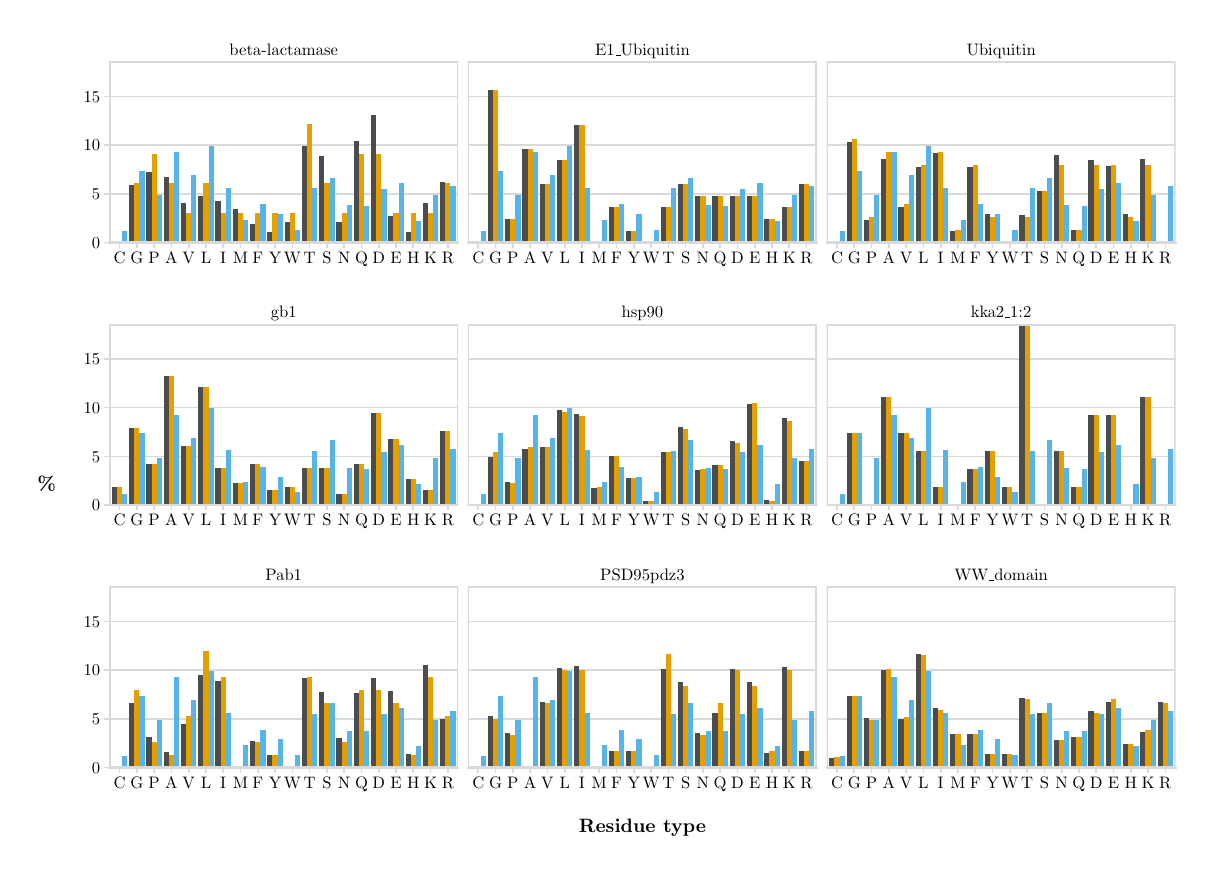
\begin{tikzpicture}[x=1pt,y=1pt]
\definecolor{fillColor}{RGB}{255,255,255}
\path[use as bounding box,fill=fillColor,fill opacity=0.00] (0,0) rectangle (418.34,295.82);
\begin{scope}
\path[clip] ( 29.46,218.05) rectangle (155.58,283.52);
\definecolor{drawColor}{gray}{0.85}

\path[draw=drawColor,line width= 0.6pt,line join=round] ( 29.46,218.18) --
	(155.58,218.18);

\path[draw=drawColor,line width= 0.6pt,line join=round] ( 29.46,235.78) --
	(155.58,235.78);

\path[draw=drawColor,line width= 0.6pt,line join=round] ( 29.46,253.39) --
	(155.58,253.39);

\path[draw=drawColor,line width= 0.6pt,line join=round] ( 29.46,271.00) --
	(155.58,271.00);
\definecolor{fillColor}{RGB}{86,180,233}

\path[fill=fillColor] ( 52.87,218.18) rectangle ( 54.75,250.79);

\path[fill=fillColor] (152.77,218.18) rectangle (154.65,238.60);

\path[fill=fillColor] (115.31,218.18) rectangle (117.18,231.56);

\path[fill=fillColor] (127.80,218.18) rectangle (129.67,237.51);

\path[fill=fillColor] ( 34.14,218.18) rectangle ( 36.01,222.33);

\path[fill=fillColor] (121.55,218.18) rectangle (123.43,231.38);

\path[fill=fillColor] (134.04,218.18) rectangle (135.92,239.87);

\path[fill=fillColor] ( 40.38,218.18) rectangle ( 42.26,244.10);

\path[fill=fillColor] (140.29,218.18) rectangle (142.16,225.89);

\path[fill=fillColor] ( 71.60,218.18) rectangle ( 73.48,238.04);

\path[fill=fillColor] ( 65.36,218.18) rectangle ( 67.23,253.08);

\path[fill=fillColor] (146.53,218.18) rectangle (148.40,235.36);

\path[fill=fillColor] ( 77.85,218.18) rectangle ( 79.72,226.49);

\path[fill=fillColor] ( 84.09,218.18) rectangle ( 85.96,231.95);

\path[fill=fillColor] ( 46.63,218.18) rectangle ( 48.50,235.36);

\path[fill=fillColor] (109.07,218.18) rectangle (110.94,241.53);

\path[fill=fillColor] (102.82,218.18) rectangle (104.70,237.72);

\path[fill=fillColor] ( 96.58,218.18) rectangle ( 98.45,222.75);

\path[fill=fillColor] ( 90.34,218.18) rectangle ( 92.21,228.39);

\path[fill=fillColor] ( 59.12,218.18) rectangle ( 60.99,242.58);
\definecolor{fillColor}{RGB}{230,159,0}

\path[fill=fillColor] ( 32.27,218.18) rectangle ( 34.14,218.18);

\path[fill=fillColor] ( 38.51,218.18) rectangle ( 40.38,239.52);

\path[fill=fillColor] ( 44.76,218.18) rectangle ( 46.63,250.19);

\path[fill=fillColor] ( 51.00,218.18) rectangle ( 52.87,239.52);

\path[fill=fillColor] ( 57.24,218.18) rectangle ( 59.12,228.85);

\path[fill=fillColor] ( 63.49,218.18) rectangle ( 65.36,239.52);

\path[fill=fillColor] ( 69.73,218.18) rectangle ( 71.60,228.85);

\path[fill=fillColor] ( 75.97,218.18) rectangle ( 77.85,228.85);

\path[fill=fillColor] ( 82.22,218.18) rectangle ( 84.09,228.85);

\path[fill=fillColor] ( 88.46,218.18) rectangle ( 90.34,228.85);

\path[fill=fillColor] ( 94.71,218.18) rectangle ( 96.58,228.85);

\path[fill=fillColor] (100.95,218.18) rectangle (102.82,260.86);

\path[fill=fillColor] (107.19,218.18) rectangle (109.07,239.52);

\path[fill=fillColor] (113.44,218.18) rectangle (115.31,228.85);

\path[fill=fillColor] (119.68,218.18) rectangle (121.55,250.19);

\path[fill=fillColor] (125.93,218.18) rectangle (127.80,250.19);

\path[fill=fillColor] (132.17,218.18) rectangle (134.04,228.85);

\path[fill=fillColor] (138.41,218.18) rectangle (140.29,228.85);

\path[fill=fillColor] (144.66,218.18) rectangle (146.53,228.85);

\path[fill=fillColor] (150.90,218.18) rectangle (152.77,239.52);
\definecolor{fillColor}{gray}{0.30}

\path[fill=fillColor] ( 30.39,218.18) rectangle ( 32.27,218.18);

\path[fill=fillColor] ( 36.64,218.18) rectangle ( 38.51,238.95);

\path[fill=fillColor] ( 42.88,218.18) rectangle ( 44.76,243.67);

\path[fill=fillColor] ( 49.13,218.18) rectangle ( 51.00,241.78);

\path[fill=fillColor] ( 55.37,218.18) rectangle ( 57.24,232.34);

\path[fill=fillColor] ( 61.61,218.18) rectangle ( 63.49,235.17);

\path[fill=fillColor] ( 67.86,218.18) rectangle ( 69.73,233.28);

\path[fill=fillColor] ( 74.10,218.18) rectangle ( 75.97,230.45);

\path[fill=fillColor] ( 80.35,218.18) rectangle ( 82.22,224.79);

\path[fill=fillColor] ( 86.59,218.18) rectangle ( 88.46,221.95);

\path[fill=fillColor] ( 92.83,218.18) rectangle ( 94.71,225.73);

\path[fill=fillColor] ( 99.08,218.18) rectangle (100.95,253.11);

\path[fill=fillColor] (105.32,218.18) rectangle (107.19,249.33);

\path[fill=fillColor] (111.56,218.18) rectangle (113.44,225.73);

\path[fill=fillColor] (117.81,218.18) rectangle (119.68,255.00);

\path[fill=fillColor] (124.05,218.18) rectangle (125.93,264.44);

\path[fill=fillColor] (130.30,218.18) rectangle (132.17,227.62);

\path[fill=fillColor] (136.54,218.18) rectangle (138.41,221.95);

\path[fill=fillColor] (142.78,218.18) rectangle (144.66,232.34);

\path[fill=fillColor] (149.03,218.18) rectangle (150.90,239.89);

\path[draw=drawColor,line width= 1.1pt,line join=round,line cap=round] ( 29.46,218.05) rectangle (155.58,283.52);
\end{scope}
\begin{scope}
\path[clip] ( 29.46,123.17) rectangle (155.58,188.65);
\definecolor{drawColor}{gray}{0.85}

\path[draw=drawColor,line width= 0.6pt,line join=round] ( 29.46,123.31) --
	(155.58,123.31);

\path[draw=drawColor,line width= 0.6pt,line join=round] ( 29.46,140.91) --
	(155.58,140.91);

\path[draw=drawColor,line width= 0.6pt,line join=round] ( 29.46,158.52) --
	(155.58,158.52);

\path[draw=drawColor,line width= 0.6pt,line join=round] ( 29.46,176.13) --
	(155.58,176.13);
\definecolor{fillColor}{RGB}{86,180,233}

\path[fill=fillColor] ( 52.87,123.31) rectangle ( 54.75,155.92);

\path[fill=fillColor] (152.77,123.31) rectangle (154.65,143.73);

\path[fill=fillColor] (115.31,123.31) rectangle (117.18,136.69);

\path[fill=fillColor] (127.80,123.31) rectangle (129.67,142.64);

\path[fill=fillColor] ( 34.14,123.31) rectangle ( 36.01,127.46);

\path[fill=fillColor] (121.55,123.31) rectangle (123.43,136.51);

\path[fill=fillColor] (134.04,123.31) rectangle (135.92,145.00);

\path[fill=fillColor] ( 40.38,123.31) rectangle ( 42.26,149.22);

\path[fill=fillColor] (140.29,123.31) rectangle (142.16,131.02);

\path[fill=fillColor] ( 71.60,123.31) rectangle ( 73.48,143.17);

\path[fill=fillColor] ( 65.36,123.31) rectangle ( 67.23,158.21);

\path[fill=fillColor] (146.53,123.31) rectangle (148.40,140.49);

\path[fill=fillColor] ( 77.85,123.31) rectangle ( 79.72,131.62);

\path[fill=fillColor] ( 84.09,123.31) rectangle ( 85.96,137.08);

\path[fill=fillColor] ( 46.63,123.31) rectangle ( 48.50,140.49);

\path[fill=fillColor] (109.07,123.31) rectangle (110.94,146.65);

\path[fill=fillColor] (102.82,123.31) rectangle (104.70,142.85);

\path[fill=fillColor] ( 96.58,123.31) rectangle ( 98.45,127.88);

\path[fill=fillColor] ( 90.34,123.31) rectangle ( 92.21,133.52);

\path[fill=fillColor] ( 59.12,123.31) rectangle ( 60.99,147.71);
\definecolor{fillColor}{RGB}{230,159,0}

\path[fill=fillColor] ( 32.27,123.31) rectangle ( 34.14,129.98);

\path[fill=fillColor] ( 38.51,123.31) rectangle ( 40.38,151.32);

\path[fill=fillColor] ( 44.76,123.31) rectangle ( 46.63,137.98);

\path[fill=fillColor] ( 51.00,123.31) rectangle ( 52.87,169.99);

\path[fill=fillColor] ( 57.24,123.31) rectangle ( 59.12,144.65);

\path[fill=fillColor] ( 63.49,123.31) rectangle ( 65.36,165.99);

\path[fill=fillColor] ( 69.73,123.31) rectangle ( 71.60,136.65);

\path[fill=fillColor] ( 75.97,123.31) rectangle ( 77.85,131.31);

\path[fill=fillColor] ( 82.22,123.31) rectangle ( 84.09,137.98);

\path[fill=fillColor] ( 88.46,123.31) rectangle ( 90.34,128.64);

\path[fill=fillColor] ( 94.71,123.31) rectangle ( 96.58,129.98);

\path[fill=fillColor] (100.95,123.31) rectangle (102.82,136.65);

\path[fill=fillColor] (107.19,123.31) rectangle (109.07,136.65);

\path[fill=fillColor] (113.44,123.31) rectangle (115.31,127.31);

\path[fill=fillColor] (119.68,123.31) rectangle (121.55,137.98);

\path[fill=fillColor] (125.93,123.31) rectangle (127.80,156.65);

\path[fill=fillColor] (132.17,123.31) rectangle (134.04,147.32);

\path[fill=fillColor] (138.41,123.31) rectangle (140.29,132.64);

\path[fill=fillColor] (144.66,123.31) rectangle (146.53,128.64);

\path[fill=fillColor] (150.90,123.31) rectangle (152.77,149.98);
\definecolor{fillColor}{gray}{0.30}

\path[fill=fillColor] ( 30.39,123.31) rectangle ( 32.27,129.98);

\path[fill=fillColor] ( 36.64,123.31) rectangle ( 38.51,151.32);

\path[fill=fillColor] ( 42.88,123.31) rectangle ( 44.76,137.98);

\path[fill=fillColor] ( 49.13,123.31) rectangle ( 51.00,169.99);

\path[fill=fillColor] ( 55.37,123.31) rectangle ( 57.24,144.65);

\path[fill=fillColor] ( 61.61,123.31) rectangle ( 63.49,165.99);

\path[fill=fillColor] ( 67.86,123.31) rectangle ( 69.73,136.65);

\path[fill=fillColor] ( 74.10,123.31) rectangle ( 75.97,131.31);

\path[fill=fillColor] ( 80.35,123.31) rectangle ( 82.22,137.98);

\path[fill=fillColor] ( 86.59,123.31) rectangle ( 88.46,128.64);

\path[fill=fillColor] ( 92.83,123.31) rectangle ( 94.71,129.98);

\path[fill=fillColor] ( 99.08,123.31) rectangle (100.95,136.65);

\path[fill=fillColor] (105.32,123.31) rectangle (107.19,136.65);

\path[fill=fillColor] (111.56,123.31) rectangle (113.44,127.31);

\path[fill=fillColor] (117.81,123.31) rectangle (119.68,137.98);

\path[fill=fillColor] (124.05,123.31) rectangle (125.93,156.65);

\path[fill=fillColor] (130.30,123.31) rectangle (132.17,147.32);

\path[fill=fillColor] (136.54,123.31) rectangle (138.41,132.64);

\path[fill=fillColor] (142.78,123.31) rectangle (144.66,128.64);

\path[fill=fillColor] (149.03,123.31) rectangle (150.90,149.98);

\path[draw=drawColor,line width= 1.1pt,line join=round,line cap=round] ( 29.46,123.17) rectangle (155.58,188.65);
\end{scope}
\begin{scope}
\path[clip] ( 29.46, 28.30) rectangle (155.58, 93.78);
\definecolor{drawColor}{gray}{0.85}

\path[draw=drawColor,line width= 0.6pt,line join=round] ( 29.46, 28.43) --
	(155.58, 28.43);

\path[draw=drawColor,line width= 0.6pt,line join=round] ( 29.46, 46.04) --
	(155.58, 46.04);

\path[draw=drawColor,line width= 0.6pt,line join=round] ( 29.46, 63.65) --
	(155.58, 63.65);

\path[draw=drawColor,line width= 0.6pt,line join=round] ( 29.46, 81.26) --
	(155.58, 81.26);
\definecolor{fillColor}{RGB}{86,180,233}

\path[fill=fillColor] ( 52.87, 28.43) rectangle ( 54.75, 61.04);

\path[fill=fillColor] (152.77, 28.43) rectangle (154.65, 48.86);

\path[fill=fillColor] (115.31, 28.43) rectangle (117.18, 41.82);

\path[fill=fillColor] (127.80, 28.43) rectangle (129.67, 47.77);

\path[fill=fillColor] ( 34.14, 28.43) rectangle ( 36.01, 32.59);

\path[fill=fillColor] (121.55, 28.43) rectangle (123.43, 41.64);

\path[fill=fillColor] (134.04, 28.43) rectangle (135.92, 50.13);

\path[fill=fillColor] ( 40.38, 28.43) rectangle ( 42.26, 54.35);

\path[fill=fillColor] (140.29, 28.43) rectangle (142.16, 36.15);

\path[fill=fillColor] ( 71.60, 28.43) rectangle ( 73.48, 48.30);

\path[fill=fillColor] ( 65.36, 28.43) rectangle ( 67.23, 63.33);

\path[fill=fillColor] (146.53, 28.43) rectangle (148.40, 45.62);

\path[fill=fillColor] ( 77.85, 28.43) rectangle ( 79.72, 36.75);

\path[fill=fillColor] ( 84.09, 28.43) rectangle ( 85.96, 42.20);

\path[fill=fillColor] ( 46.63, 28.43) rectangle ( 48.50, 45.62);

\path[fill=fillColor] (109.07, 28.43) rectangle (110.94, 51.78);

\path[fill=fillColor] (102.82, 28.43) rectangle (104.70, 47.98);

\path[fill=fillColor] ( 96.58, 28.43) rectangle ( 98.45, 33.01);

\path[fill=fillColor] ( 90.34, 28.43) rectangle ( 92.21, 38.65);

\path[fill=fillColor] ( 59.12, 28.43) rectangle ( 60.99, 52.84);
\definecolor{fillColor}{RGB}{230,159,0}

\path[fill=fillColor] ( 32.27, 28.43) rectangle ( 34.14, 28.43);

\path[fill=fillColor] ( 38.51, 28.43) rectangle ( 40.38, 56.61);

\path[fill=fillColor] ( 44.76, 28.43) rectangle ( 46.63, 37.83);

\path[fill=fillColor] ( 51.00, 28.43) rectangle ( 52.87, 33.13);

\path[fill=fillColor] ( 57.24, 28.43) rectangle ( 59.12, 47.22);

\path[fill=fillColor] ( 63.49, 28.43) rectangle ( 65.36, 70.69);

\path[fill=fillColor] ( 69.73, 28.43) rectangle ( 71.60, 61.30);

\path[fill=fillColor] ( 75.97, 28.43) rectangle ( 77.85, 28.43);

\path[fill=fillColor] ( 82.22, 28.43) rectangle ( 84.09, 37.83);

\path[fill=fillColor] ( 88.46, 28.43) rectangle ( 90.34, 33.13);

\path[fill=fillColor] ( 94.71, 28.43) rectangle ( 96.58, 28.43);

\path[fill=fillColor] (100.95, 28.43) rectangle (102.82, 61.30);

\path[fill=fillColor] (107.19, 28.43) rectangle (109.07, 51.91);

\path[fill=fillColor] (113.44, 28.43) rectangle (115.31, 37.83);

\path[fill=fillColor] (119.68, 28.43) rectangle (121.55, 56.61);

\path[fill=fillColor] (125.93, 28.43) rectangle (127.80, 56.61);

\path[fill=fillColor] (132.17, 28.43) rectangle (134.04, 51.91);

\path[fill=fillColor] (138.41, 28.43) rectangle (140.29, 33.13);

\path[fill=fillColor] (144.66, 28.43) rectangle (146.53, 61.30);

\path[fill=fillColor] (150.90, 28.43) rectangle (152.77, 47.22);
\definecolor{fillColor}{gray}{0.30}

\path[fill=fillColor] ( 30.39, 28.43) rectangle ( 32.27, 28.43);

\path[fill=fillColor] ( 36.64, 28.43) rectangle ( 38.51, 51.78);

\path[fill=fillColor] ( 42.88, 28.43) rectangle ( 44.76, 39.55);

\path[fill=fillColor] ( 49.13, 28.43) rectangle ( 51.00, 33.99);

\path[fill=fillColor] ( 55.37, 28.43) rectangle ( 57.24, 44.28);

\path[fill=fillColor] ( 61.61, 28.43) rectangle ( 63.49, 62.07);

\path[fill=fillColor] ( 67.86, 28.43) rectangle ( 69.73, 59.84);

\path[fill=fillColor] ( 74.10, 28.43) rectangle ( 75.97, 28.43);

\path[fill=fillColor] ( 80.35, 28.43) rectangle ( 82.22, 38.16);

\path[fill=fillColor] ( 86.59, 28.43) rectangle ( 88.46, 32.88);

\path[fill=fillColor] ( 92.83, 28.43) rectangle ( 94.71, 28.43);

\path[fill=fillColor] ( 99.08, 28.43) rectangle (100.95, 60.95);

\path[fill=fillColor] (105.32, 28.43) rectangle (107.19, 55.67);

\path[fill=fillColor] (111.56, 28.43) rectangle (113.44, 39.27);

\path[fill=fillColor] (117.81, 28.43) rectangle (119.68, 55.40);

\path[fill=fillColor] (124.05, 28.43) rectangle (125.93, 60.68);

\path[fill=fillColor] (130.30, 28.43) rectangle (132.17, 55.95);

\path[fill=fillColor] (136.54, 28.43) rectangle (138.41, 33.44);

\path[fill=fillColor] (142.78, 28.43) rectangle (144.66, 65.68);

\path[fill=fillColor] (149.03, 28.43) rectangle (150.90, 45.95);

\path[draw=drawColor,line width= 1.1pt,line join=round,line cap=round] ( 29.46, 28.30) rectangle (155.58, 93.78);
\end{scope}
\begin{scope}
\path[clip] (159.08,218.05) rectangle (285.21,283.52);
\definecolor{drawColor}{gray}{0.85}

\path[draw=drawColor,line width= 0.6pt,line join=round] (159.08,218.18) --
	(285.21,218.18);

\path[draw=drawColor,line width= 0.6pt,line join=round] (159.08,235.78) --
	(285.21,235.78);

\path[draw=drawColor,line width= 0.6pt,line join=round] (159.08,253.39) --
	(285.21,253.39);

\path[draw=drawColor,line width= 0.6pt,line join=round] (159.08,271.00) --
	(285.21,271.00);
\definecolor{fillColor}{RGB}{86,180,233}

\path[fill=fillColor] (182.50,218.18) rectangle (184.37,250.79);

\path[fill=fillColor] (282.40,218.18) rectangle (284.27,238.60);

\path[fill=fillColor] (244.94,218.18) rectangle (246.81,231.56);

\path[fill=fillColor] (257.42,218.18) rectangle (259.30,237.51);

\path[fill=fillColor] (163.77,218.18) rectangle (165.64,222.33);

\path[fill=fillColor] (251.18,218.18) rectangle (253.05,231.38);

\path[fill=fillColor] (263.67,218.18) rectangle (265.54,239.87);

\path[fill=fillColor] (170.01,218.18) rectangle (171.88,244.10);

\path[fill=fillColor] (269.91,218.18) rectangle (271.79,225.89);

\path[fill=fillColor] (201.23,218.18) rectangle (203.10,238.04);

\path[fill=fillColor] (194.99,218.18) rectangle (196.86,253.08);

\path[fill=fillColor] (276.16,218.18) rectangle (278.03,235.36);

\path[fill=fillColor] (207.47,218.18) rectangle (209.35,226.49);

\path[fill=fillColor] (213.72,218.18) rectangle (215.59,231.95);

\path[fill=fillColor] (176.25,218.18) rectangle (178.13,235.36);

\path[fill=fillColor] (238.69,218.18) rectangle (240.57,241.53);

\path[fill=fillColor] (232.45,218.18) rectangle (234.32,237.72);

\path[fill=fillColor] (226.21,218.18) rectangle (228.08,222.75);

\path[fill=fillColor] (219.96,218.18) rectangle (221.83,228.39);

\path[fill=fillColor] (188.74,218.18) rectangle (190.62,242.58);
\definecolor{fillColor}{RGB}{230,159,0}

\path[fill=fillColor] (161.89,218.18) rectangle (163.77,218.18);

\path[fill=fillColor] (168.14,218.18) rectangle (170.01,273.34);

\path[fill=fillColor] (174.38,218.18) rectangle (176.25,226.66);

\path[fill=fillColor] (180.63,218.18) rectangle (182.50,252.12);

\path[fill=fillColor] (186.87,218.18) rectangle (188.74,239.39);

\path[fill=fillColor] (193.11,218.18) rectangle (194.99,247.88);

\path[fill=fillColor] (199.36,218.18) rectangle (201.23,260.61);

\path[fill=fillColor] (205.60,218.18) rectangle (207.47,218.18);

\path[fill=fillColor] (211.84,218.18) rectangle (213.72,230.91);

\path[fill=fillColor] (218.09,218.18) rectangle (219.96,222.42);

\path[fill=fillColor] (224.33,218.18) rectangle (226.21,218.18);

\path[fill=fillColor] (230.58,218.18) rectangle (232.45,230.91);

\path[fill=fillColor] (236.82,218.18) rectangle (238.69,239.39);

\path[fill=fillColor] (243.06,218.18) rectangle (244.94,235.15);

\path[fill=fillColor] (249.31,218.18) rectangle (251.18,235.15);

\path[fill=fillColor] (255.55,218.18) rectangle (257.42,235.15);

\path[fill=fillColor] (261.80,218.18) rectangle (263.67,235.15);

\path[fill=fillColor] (268.04,218.18) rectangle (269.91,226.66);

\path[fill=fillColor] (274.28,218.18) rectangle (276.16,230.91);

\path[fill=fillColor] (280.53,218.18) rectangle (282.40,239.39);
\definecolor{fillColor}{gray}{0.30}

\path[fill=fillColor] (160.02,218.18) rectangle (161.89,218.18);

\path[fill=fillColor] (166.26,218.18) rectangle (168.14,273.34);

\path[fill=fillColor] (172.51,218.18) rectangle (174.38,226.66);

\path[fill=fillColor] (178.75,218.18) rectangle (180.63,252.12);

\path[fill=fillColor] (185.00,218.18) rectangle (186.87,239.39);

\path[fill=fillColor] (191.24,218.18) rectangle (193.11,247.88);

\path[fill=fillColor] (197.48,218.18) rectangle (199.36,260.61);

\path[fill=fillColor] (203.73,218.18) rectangle (205.60,218.18);

\path[fill=fillColor] (209.97,218.18) rectangle (211.84,230.91);

\path[fill=fillColor] (216.22,218.18) rectangle (218.09,222.42);

\path[fill=fillColor] (222.46,218.18) rectangle (224.33,218.18);

\path[fill=fillColor] (228.70,218.18) rectangle (230.58,230.91);

\path[fill=fillColor] (234.95,218.18) rectangle (236.82,239.39);

\path[fill=fillColor] (241.19,218.18) rectangle (243.06,235.15);

\path[fill=fillColor] (247.43,218.18) rectangle (249.31,235.15);

\path[fill=fillColor] (253.68,218.18) rectangle (255.55,235.15);

\path[fill=fillColor] (259.92,218.18) rectangle (261.80,235.15);

\path[fill=fillColor] (266.17,218.18) rectangle (268.04,226.66);

\path[fill=fillColor] (272.41,218.18) rectangle (274.28,230.91);

\path[fill=fillColor] (278.65,218.18) rectangle (280.53,239.39);

\path[draw=drawColor,line width= 1.1pt,line join=round,line cap=round] (159.08,218.05) rectangle (285.21,283.52);
\end{scope}
\begin{scope}
\path[clip] (159.08,123.17) rectangle (285.21,188.65);
\definecolor{drawColor}{gray}{0.85}

\path[draw=drawColor,line width= 0.6pt,line join=round] (159.08,123.31) --
	(285.21,123.31);

\path[draw=drawColor,line width= 0.6pt,line join=round] (159.08,140.91) --
	(285.21,140.91);

\path[draw=drawColor,line width= 0.6pt,line join=round] (159.08,158.52) --
	(285.21,158.52);

\path[draw=drawColor,line width= 0.6pt,line join=round] (159.08,176.13) --
	(285.21,176.13);
\definecolor{fillColor}{RGB}{86,180,233}

\path[fill=fillColor] (182.50,123.31) rectangle (184.37,155.92);

\path[fill=fillColor] (282.40,123.31) rectangle (284.27,143.73);

\path[fill=fillColor] (244.94,123.31) rectangle (246.81,136.69);

\path[fill=fillColor] (257.42,123.31) rectangle (259.30,142.64);

\path[fill=fillColor] (163.77,123.31) rectangle (165.64,127.46);

\path[fill=fillColor] (251.18,123.31) rectangle (253.05,136.51);

\path[fill=fillColor] (263.67,123.31) rectangle (265.54,145.00);

\path[fill=fillColor] (170.01,123.31) rectangle (171.88,149.22);

\path[fill=fillColor] (269.91,123.31) rectangle (271.79,131.02);

\path[fill=fillColor] (201.23,123.31) rectangle (203.10,143.17);

\path[fill=fillColor] (194.99,123.31) rectangle (196.86,158.21);

\path[fill=fillColor] (276.16,123.31) rectangle (278.03,140.49);

\path[fill=fillColor] (207.47,123.31) rectangle (209.35,131.62);

\path[fill=fillColor] (213.72,123.31) rectangle (215.59,137.08);

\path[fill=fillColor] (176.25,123.31) rectangle (178.13,140.49);

\path[fill=fillColor] (238.69,123.31) rectangle (240.57,146.65);

\path[fill=fillColor] (232.45,123.31) rectangle (234.32,142.85);

\path[fill=fillColor] (226.21,123.31) rectangle (228.08,127.88);

\path[fill=fillColor] (219.96,123.31) rectangle (221.83,133.52);

\path[fill=fillColor] (188.74,123.31) rectangle (190.62,147.71);
\definecolor{fillColor}{RGB}{230,159,0}

\path[fill=fillColor] (161.89,123.31) rectangle (163.77,123.31);

\path[fill=fillColor] (168.14,123.31) rectangle (170.01,142.60);

\path[fill=fillColor] (174.38,123.31) rectangle (176.25,131.35);

\path[fill=fillColor] (180.63,123.31) rectangle (182.50,144.21);

\path[fill=fillColor] (186.87,123.31) rectangle (188.74,144.21);

\path[fill=fillColor] (193.11,123.31) rectangle (194.99,157.07);

\path[fill=fillColor] (199.36,123.31) rectangle (201.23,155.47);

\path[fill=fillColor] (205.60,123.31) rectangle (207.47,129.74);

\path[fill=fillColor] (211.84,123.31) rectangle (213.72,140.99);

\path[fill=fillColor] (218.09,123.31) rectangle (219.96,132.95);

\path[fill=fillColor] (224.33,123.31) rectangle (226.21,124.91);

\path[fill=fillColor] (230.58,123.31) rectangle (232.45,142.60);

\path[fill=fillColor] (236.82,123.31) rectangle (238.69,150.64);

\path[fill=fillColor] (243.06,123.31) rectangle (244.94,136.17);

\path[fill=fillColor] (249.31,123.31) rectangle (251.18,137.78);

\path[fill=fillColor] (255.55,123.31) rectangle (257.42,145.82);

\path[fill=fillColor] (261.80,123.31) rectangle (263.67,160.29);

\path[fill=fillColor] (268.04,123.31) rectangle (269.91,124.91);

\path[fill=fillColor] (274.28,123.31) rectangle (276.16,153.86);

\path[fill=fillColor] (280.53,123.31) rectangle (282.40,139.39);
\definecolor{fillColor}{gray}{0.30}

\path[fill=fillColor] (160.02,123.31) rectangle (161.89,123.31);

\path[fill=fillColor] (166.26,123.31) rectangle (168.14,140.70);

\path[fill=fillColor] (172.51,123.31) rectangle (174.38,131.55);

\path[fill=fillColor] (178.75,123.31) rectangle (180.63,143.61);

\path[fill=fillColor] (185.00,123.31) rectangle (186.87,144.28);

\path[fill=fillColor] (191.24,123.31) rectangle (193.11,157.51);

\path[fill=fillColor] (197.48,123.31) rectangle (199.36,156.27);

\path[fill=fillColor] (203.73,123.31) rectangle (205.60,129.30);

\path[fill=fillColor] (209.97,123.31) rectangle (211.84,140.95);

\path[fill=fillColor] (216.22,123.31) rectangle (218.09,133.04);

\path[fill=fillColor] (222.46,123.31) rectangle (224.33,124.89);

\path[fill=fillColor] (228.70,123.31) rectangle (230.58,142.53);

\path[fill=fillColor] (234.95,123.31) rectangle (236.82,151.36);

\path[fill=fillColor] (241.19,123.31) rectangle (243.06,136.04);

\path[fill=fillColor] (247.43,123.31) rectangle (249.31,137.95);

\path[fill=fillColor] (253.68,123.31) rectangle (255.55,146.53);

\path[fill=fillColor] (259.92,123.31) rectangle (261.80,159.68);

\path[fill=fillColor] (266.17,123.31) rectangle (268.04,124.97);

\path[fill=fillColor] (272.41,123.31) rectangle (274.28,154.68);

\path[fill=fillColor] (278.65,123.31) rectangle (280.53,139.12);

\path[draw=drawColor,line width= 1.1pt,line join=round,line cap=round] (159.08,123.17) rectangle (285.21,188.65);
\end{scope}
\begin{scope}
\path[clip] (159.08, 28.30) rectangle (285.21, 93.78);
\definecolor{drawColor}{gray}{0.85}

\path[draw=drawColor,line width= 0.6pt,line join=round] (159.08, 28.43) --
	(285.21, 28.43);

\path[draw=drawColor,line width= 0.6pt,line join=round] (159.08, 46.04) --
	(285.21, 46.04);

\path[draw=drawColor,line width= 0.6pt,line join=round] (159.08, 63.65) --
	(285.21, 63.65);

\path[draw=drawColor,line width= 0.6pt,line join=round] (159.08, 81.26) --
	(285.21, 81.26);
\definecolor{fillColor}{RGB}{86,180,233}

\path[fill=fillColor] (182.50, 28.43) rectangle (184.37, 61.04);

\path[fill=fillColor] (282.40, 28.43) rectangle (284.27, 48.86);

\path[fill=fillColor] (244.94, 28.43) rectangle (246.81, 41.82);

\path[fill=fillColor] (257.42, 28.43) rectangle (259.30, 47.77);

\path[fill=fillColor] (163.77, 28.43) rectangle (165.64, 32.59);

\path[fill=fillColor] (251.18, 28.43) rectangle (253.05, 41.64);

\path[fill=fillColor] (263.67, 28.43) rectangle (265.54, 50.13);

\path[fill=fillColor] (170.01, 28.43) rectangle (171.88, 54.35);

\path[fill=fillColor] (269.91, 28.43) rectangle (271.79, 36.15);

\path[fill=fillColor] (201.23, 28.43) rectangle (203.10, 48.30);

\path[fill=fillColor] (194.99, 28.43) rectangle (196.86, 63.33);

\path[fill=fillColor] (276.16, 28.43) rectangle (278.03, 45.62);

\path[fill=fillColor] (207.47, 28.43) rectangle (209.35, 36.75);

\path[fill=fillColor] (213.72, 28.43) rectangle (215.59, 42.20);

\path[fill=fillColor] (176.25, 28.43) rectangle (178.13, 45.62);

\path[fill=fillColor] (238.69, 28.43) rectangle (240.57, 51.78);

\path[fill=fillColor] (232.45, 28.43) rectangle (234.32, 47.98);

\path[fill=fillColor] (226.21, 28.43) rectangle (228.08, 33.01);

\path[fill=fillColor] (219.96, 28.43) rectangle (221.83, 38.65);

\path[fill=fillColor] (188.74, 28.43) rectangle (190.62, 52.84);
\definecolor{fillColor}{RGB}{230,159,0}

\path[fill=fillColor] (161.89, 28.43) rectangle (163.77, 28.43);

\path[fill=fillColor] (168.14, 28.43) rectangle (170.01, 46.04);

\path[fill=fillColor] (174.38, 28.43) rectangle (176.25, 40.17);

\path[fill=fillColor] (180.63, 28.43) rectangle (182.50, 28.43);

\path[fill=fillColor] (186.87, 28.43) rectangle (188.74, 51.91);

\path[fill=fillColor] (193.11, 28.43) rectangle (194.99, 63.65);

\path[fill=fillColor] (199.36, 28.43) rectangle (201.23, 63.65);

\path[fill=fillColor] (205.60, 28.43) rectangle (207.47, 28.43);

\path[fill=fillColor] (211.84, 28.43) rectangle (213.72, 34.30);

\path[fill=fillColor] (218.09, 28.43) rectangle (219.96, 34.30);

\path[fill=fillColor] (224.33, 28.43) rectangle (226.21, 28.43);

\path[fill=fillColor] (230.58, 28.43) rectangle (232.45, 69.52);

\path[fill=fillColor] (236.82, 28.43) rectangle (238.69, 57.78);

\path[fill=fillColor] (243.06, 28.43) rectangle (244.94, 40.17);

\path[fill=fillColor] (249.31, 28.43) rectangle (251.18, 51.91);

\path[fill=fillColor] (255.55, 28.43) rectangle (257.42, 63.65);

\path[fill=fillColor] (261.80, 28.43) rectangle (263.67, 57.78);

\path[fill=fillColor] (268.04, 28.43) rectangle (269.91, 34.30);

\path[fill=fillColor] (274.28, 28.43) rectangle (276.16, 63.65);

\path[fill=fillColor] (280.53, 28.43) rectangle (282.40, 34.30);
\definecolor{fillColor}{gray}{0.30}

\path[fill=fillColor] (160.02, 28.43) rectangle (161.89, 28.43);

\path[fill=fillColor] (166.26, 28.43) rectangle (168.14, 46.94);

\path[fill=fillColor] (172.51, 28.43) rectangle (174.38, 40.77);

\path[fill=fillColor] (178.75, 28.43) rectangle (180.63, 28.43);

\path[fill=fillColor] (185.00, 28.43) rectangle (186.87, 52.18);

\path[fill=fillColor] (191.24, 28.43) rectangle (193.11, 64.51);

\path[fill=fillColor] (197.48, 28.43) rectangle (199.36, 65.13);

\path[fill=fillColor] (203.73, 28.43) rectangle (205.60, 28.43);

\path[fill=fillColor] (209.97, 28.43) rectangle (211.84, 34.60);

\path[fill=fillColor] (216.22, 28.43) rectangle (218.09, 34.60);

\path[fill=fillColor] (222.46, 28.43) rectangle (224.33, 28.43);

\path[fill=fillColor] (228.70, 28.43) rectangle (230.58, 63.90);

\path[fill=fillColor] (234.95, 28.43) rectangle (236.82, 59.27);

\path[fill=fillColor] (241.19, 28.43) rectangle (243.06, 40.77);

\path[fill=fillColor] (247.43, 28.43) rectangle (249.31, 48.17);

\path[fill=fillColor] (253.68, 28.43) rectangle (255.55, 64.21);

\path[fill=fillColor] (259.92, 28.43) rectangle (261.80, 59.27);

\path[fill=fillColor] (266.17, 28.43) rectangle (268.04, 33.68);

\path[fill=fillColor] (272.41, 28.43) rectangle (274.28, 64.82);

\path[fill=fillColor] (278.65, 28.43) rectangle (280.53, 34.29);

\path[draw=drawColor,line width= 1.1pt,line join=round,line cap=round] (159.08, 28.30) rectangle (285.21, 93.78);
\end{scope}
\begin{scope}
\path[clip] (288.71,218.05) rectangle (414.84,283.52);
\definecolor{drawColor}{gray}{0.85}

\path[draw=drawColor,line width= 0.6pt,line join=round] (288.71,218.18) --
	(414.84,218.18);

\path[draw=drawColor,line width= 0.6pt,line join=round] (288.71,235.78) --
	(414.84,235.78);

\path[draw=drawColor,line width= 0.6pt,line join=round] (288.71,253.39) --
	(414.84,253.39);

\path[draw=drawColor,line width= 0.6pt,line join=round] (288.71,271.00) --
	(414.84,271.00);
\definecolor{fillColor}{RGB}{86,180,233}

\path[fill=fillColor] (312.12,218.18) rectangle (314.00,250.79);

\path[fill=fillColor] (412.03,218.18) rectangle (413.90,238.60);

\path[fill=fillColor] (374.56,218.18) rectangle (376.44,231.56);

\path[fill=fillColor] (387.05,218.18) rectangle (388.92,237.51);

\path[fill=fillColor] (293.39,218.18) rectangle (295.27,222.33);

\path[fill=fillColor] (380.81,218.18) rectangle (382.68,231.38);

\path[fill=fillColor] (393.29,218.18) rectangle (395.17,239.87);

\path[fill=fillColor] (299.64,218.18) rectangle (301.51,244.10);

\path[fill=fillColor] (399.54,218.18) rectangle (401.41,225.89);

\path[fill=fillColor] (330.86,218.18) rectangle (332.73,238.04);

\path[fill=fillColor] (324.61,218.18) rectangle (326.49,253.08);

\path[fill=fillColor] (405.78,218.18) rectangle (407.66,235.36);

\path[fill=fillColor] (337.10,218.18) rectangle (338.97,226.49);

\path[fill=fillColor] (343.34,218.18) rectangle (345.22,231.95);

\path[fill=fillColor] (305.88,218.18) rectangle (307.75,235.36);

\path[fill=fillColor] (368.32,218.18) rectangle (370.19,241.53);

\path[fill=fillColor] (362.08,218.18) rectangle (363.95,237.72);

\path[fill=fillColor] (355.83,218.18) rectangle (357.70,222.75);

\path[fill=fillColor] (349.59,218.18) rectangle (351.46,228.39);

\path[fill=fillColor] (318.37,218.18) rectangle (320.24,242.58);
\definecolor{fillColor}{RGB}{230,159,0}

\path[fill=fillColor] (291.52,218.18) rectangle (293.39,218.18);

\path[fill=fillColor] (297.76,218.18) rectangle (299.64,255.74);

\path[fill=fillColor] (304.01,218.18) rectangle (305.88,227.57);

\path[fill=fillColor] (310.25,218.18) rectangle (312.12,251.05);

\path[fill=fillColor] (316.49,218.18) rectangle (318.37,232.26);

\path[fill=fillColor] (322.74,218.18) rectangle (324.61,246.35);

\path[fill=fillColor] (328.98,218.18) rectangle (330.86,251.05);

\path[fill=fillColor] (335.23,218.18) rectangle (337.10,222.87);

\path[fill=fillColor] (341.47,218.18) rectangle (343.34,246.35);

\path[fill=fillColor] (347.71,218.18) rectangle (349.59,227.57);

\path[fill=fillColor] (353.96,218.18) rectangle (355.83,218.18);

\path[fill=fillColor] (360.20,218.18) rectangle (362.08,227.57);

\path[fill=fillColor] (366.45,218.18) rectangle (368.32,236.96);

\path[fill=fillColor] (372.69,218.18) rectangle (374.56,246.35);

\path[fill=fillColor] (378.93,218.18) rectangle (380.81,222.87);

\path[fill=fillColor] (385.18,218.18) rectangle (387.05,246.35);

\path[fill=fillColor] (391.42,218.18) rectangle (393.29,246.35);

\path[fill=fillColor] (397.67,218.18) rectangle (399.54,227.57);

\path[fill=fillColor] (403.91,218.18) rectangle (405.78,246.35);

\path[fill=fillColor] (410.15,218.18) rectangle (412.03,218.18);
\definecolor{fillColor}{gray}{0.30}

\path[fill=fillColor] (289.65,218.18) rectangle (291.52,218.18);

\path[fill=fillColor] (295.89,218.18) rectangle (297.76,254.55);

\path[fill=fillColor] (302.13,218.18) rectangle (304.01,226.26);

\path[fill=fillColor] (308.38,218.18) rectangle (310.25,248.49);

\path[fill=fillColor] (314.62,218.18) rectangle (316.49,231.17);

\path[fill=fillColor] (320.87,218.18) rectangle (322.74,245.31);

\path[fill=fillColor] (327.11,218.18) rectangle (328.98,250.51);

\path[fill=fillColor] (333.35,218.18) rectangle (335.23,222.51);

\path[fill=fillColor] (339.60,218.18) rectangle (341.47,245.31);

\path[fill=fillColor] (345.84,218.18) rectangle (347.71,228.57);

\path[fill=fillColor] (352.08,218.18) rectangle (353.96,218.18);

\path[fill=fillColor] (358.33,218.18) rectangle (360.20,228.28);

\path[fill=fillColor] (364.57,218.18) rectangle (366.45,236.94);

\path[fill=fillColor] (370.82,218.18) rectangle (372.69,249.64);

\path[fill=fillColor] (377.06,218.18) rectangle (378.93,222.80);

\path[fill=fillColor] (383.30,218.18) rectangle (385.18,247.91);

\path[fill=fillColor] (389.55,218.18) rectangle (391.42,245.89);

\path[fill=fillColor] (395.79,218.18) rectangle (397.67,228.57);

\path[fill=fillColor] (402.04,218.18) rectangle (403.91,248.49);

\path[fill=fillColor] (408.28,218.18) rectangle (410.15,218.18);

\path[draw=drawColor,line width= 1.1pt,line join=round,line cap=round] (288.71,218.05) rectangle (414.84,283.52);
\end{scope}
\begin{scope}
\path[clip] (288.71,123.17) rectangle (414.84,188.65);
\definecolor{drawColor}{gray}{0.85}

\path[draw=drawColor,line width= 0.6pt,line join=round] (288.71,123.31) --
	(414.84,123.31);

\path[draw=drawColor,line width= 0.6pt,line join=round] (288.71,140.91) --
	(414.84,140.91);

\path[draw=drawColor,line width= 0.6pt,line join=round] (288.71,158.52) --
	(414.84,158.52);

\path[draw=drawColor,line width= 0.6pt,line join=round] (288.71,176.13) --
	(414.84,176.13);
\definecolor{fillColor}{RGB}{86,180,233}

\path[fill=fillColor] (312.12,123.31) rectangle (314.00,155.92);

\path[fill=fillColor] (412.03,123.31) rectangle (413.90,143.73);

\path[fill=fillColor] (374.56,123.31) rectangle (376.44,136.69);

\path[fill=fillColor] (387.05,123.31) rectangle (388.92,142.64);

\path[fill=fillColor] (293.39,123.31) rectangle (295.27,127.46);

\path[fill=fillColor] (380.81,123.31) rectangle (382.68,136.51);

\path[fill=fillColor] (393.29,123.31) rectangle (395.17,145.00);

\path[fill=fillColor] (299.64,123.31) rectangle (301.51,149.22);

\path[fill=fillColor] (399.54,123.31) rectangle (401.41,131.02);

\path[fill=fillColor] (330.86,123.31) rectangle (332.73,143.17);

\path[fill=fillColor] (324.61,123.31) rectangle (326.49,158.21);

\path[fill=fillColor] (405.78,123.31) rectangle (407.66,140.49);

\path[fill=fillColor] (337.10,123.31) rectangle (338.97,131.62);

\path[fill=fillColor] (343.34,123.31) rectangle (345.22,137.08);

\path[fill=fillColor] (305.88,123.31) rectangle (307.75,140.49);

\path[fill=fillColor] (368.32,123.31) rectangle (370.19,146.65);

\path[fill=fillColor] (362.08,123.31) rectangle (363.95,142.85);

\path[fill=fillColor] (355.83,123.31) rectangle (357.70,127.88);

\path[fill=fillColor] (349.59,123.31) rectangle (351.46,133.52);

\path[fill=fillColor] (318.37,123.31) rectangle (320.24,147.71);
\definecolor{fillColor}{RGB}{230,159,0}

\path[fill=fillColor] (291.52,123.31) rectangle (293.39,123.31);

\path[fill=fillColor] (297.76,123.31) rectangle (299.64,149.39);

\path[fill=fillColor] (304.01,123.31) rectangle (305.88,123.31);

\path[fill=fillColor] (310.25,123.31) rectangle (312.12,162.44);

\path[fill=fillColor] (316.49,123.31) rectangle (318.37,149.39);

\path[fill=fillColor] (322.74,123.31) rectangle (324.61,142.87);

\path[fill=fillColor] (328.98,123.31) rectangle (330.86,129.83);

\path[fill=fillColor] (335.23,123.31) rectangle (337.10,123.31);

\path[fill=fillColor] (341.47,123.31) rectangle (343.34,136.35);

\path[fill=fillColor] (347.71,123.31) rectangle (349.59,142.87);

\path[fill=fillColor] (353.96,123.31) rectangle (355.83,129.83);

\path[fill=fillColor] (360.20,123.31) rectangle (362.08,188.52);

\path[fill=fillColor] (366.45,123.31) rectangle (368.32,123.31);

\path[fill=fillColor] (372.69,123.31) rectangle (374.56,142.87);

\path[fill=fillColor] (378.93,123.31) rectangle (380.81,129.83);

\path[fill=fillColor] (385.18,123.31) rectangle (387.05,155.91);

\path[fill=fillColor] (391.42,123.31) rectangle (393.29,155.91);

\path[fill=fillColor] (397.67,123.31) rectangle (399.54,123.31);

\path[fill=fillColor] (403.91,123.31) rectangle (405.78,162.44);

\path[fill=fillColor] (410.15,123.31) rectangle (412.03,123.31);
\definecolor{fillColor}{gray}{0.30}

\path[fill=fillColor] (289.65,123.31) rectangle (291.52,123.31);

\path[fill=fillColor] (295.89,123.31) rectangle (297.76,149.39);

\path[fill=fillColor] (302.13,123.31) rectangle (304.01,123.31);

\path[fill=fillColor] (308.38,123.31) rectangle (310.25,162.44);

\path[fill=fillColor] (314.62,123.31) rectangle (316.49,149.39);

\path[fill=fillColor] (320.87,123.31) rectangle (322.74,142.87);

\path[fill=fillColor] (327.11,123.31) rectangle (328.98,129.83);

\path[fill=fillColor] (333.35,123.31) rectangle (335.23,123.31);

\path[fill=fillColor] (339.60,123.31) rectangle (341.47,136.35);

\path[fill=fillColor] (345.84,123.31) rectangle (347.71,142.87);

\path[fill=fillColor] (352.08,123.31) rectangle (353.96,129.83);

\path[fill=fillColor] (358.33,123.31) rectangle (360.20,188.52);

\path[fill=fillColor] (364.57,123.31) rectangle (366.45,123.31);

\path[fill=fillColor] (370.82,123.31) rectangle (372.69,142.87);

\path[fill=fillColor] (377.06,123.31) rectangle (378.93,129.83);

\path[fill=fillColor] (383.30,123.31) rectangle (385.18,155.91);

\path[fill=fillColor] (389.55,123.31) rectangle (391.42,155.91);

\path[fill=fillColor] (395.79,123.31) rectangle (397.67,123.31);

\path[fill=fillColor] (402.04,123.31) rectangle (403.91,162.44);

\path[fill=fillColor] (408.28,123.31) rectangle (410.15,123.31);

\path[draw=drawColor,line width= 1.1pt,line join=round,line cap=round] (288.71,123.17) rectangle (414.84,188.65);
\end{scope}
\begin{scope}
\path[clip] (288.71, 28.30) rectangle (414.84, 93.78);
\definecolor{drawColor}{gray}{0.85}

\path[draw=drawColor,line width= 0.6pt,line join=round] (288.71, 28.43) --
	(414.84, 28.43);

\path[draw=drawColor,line width= 0.6pt,line join=round] (288.71, 46.04) --
	(414.84, 46.04);

\path[draw=drawColor,line width= 0.6pt,line join=round] (288.71, 63.65) --
	(414.84, 63.65);

\path[draw=drawColor,line width= 0.6pt,line join=round] (288.71, 81.26) --
	(414.84, 81.26);
\definecolor{fillColor}{RGB}{86,180,233}

\path[fill=fillColor] (312.12, 28.43) rectangle (314.00, 61.04);

\path[fill=fillColor] (412.03, 28.43) rectangle (413.90, 48.86);

\path[fill=fillColor] (374.56, 28.43) rectangle (376.44, 41.82);

\path[fill=fillColor] (387.05, 28.43) rectangle (388.92, 47.77);

\path[fill=fillColor] (293.39, 28.43) rectangle (295.27, 32.59);

\path[fill=fillColor] (380.81, 28.43) rectangle (382.68, 41.64);

\path[fill=fillColor] (393.29, 28.43) rectangle (395.17, 50.13);

\path[fill=fillColor] (299.64, 28.43) rectangle (301.51, 54.35);

\path[fill=fillColor] (399.54, 28.43) rectangle (401.41, 36.15);

\path[fill=fillColor] (330.86, 28.43) rectangle (332.73, 48.30);

\path[fill=fillColor] (324.61, 28.43) rectangle (326.49, 63.33);

\path[fill=fillColor] (405.78, 28.43) rectangle (407.66, 45.62);

\path[fill=fillColor] (337.10, 28.43) rectangle (338.97, 36.75);

\path[fill=fillColor] (343.34, 28.43) rectangle (345.22, 42.20);

\path[fill=fillColor] (305.88, 28.43) rectangle (307.75, 45.62);

\path[fill=fillColor] (368.32, 28.43) rectangle (370.19, 51.78);

\path[fill=fillColor] (362.08, 28.43) rectangle (363.95, 47.98);

\path[fill=fillColor] (355.83, 28.43) rectangle (357.70, 33.01);

\path[fill=fillColor] (349.59, 28.43) rectangle (351.46, 38.65);

\path[fill=fillColor] (318.37, 28.43) rectangle (320.24, 52.84);
\definecolor{fillColor}{RGB}{230,159,0}

\path[fill=fillColor] (291.52, 28.43) rectangle (293.39, 32.13);

\path[fill=fillColor] (297.76, 28.43) rectangle (299.64, 54.29);

\path[fill=fillColor] (304.01, 28.43) rectangle (305.88, 45.67);

\path[fill=fillColor] (310.25, 28.43) rectangle (312.12, 64.14);

\path[fill=fillColor] (316.49, 28.43) rectangle (318.37, 46.90);

\path[fill=fillColor] (322.74, 28.43) rectangle (324.61, 69.07);

\path[fill=fillColor] (328.98, 28.43) rectangle (330.86, 49.37);

\path[fill=fillColor] (335.23, 28.43) rectangle (337.10, 40.75);

\path[fill=fillColor] (341.47, 28.43) rectangle (343.34, 40.75);

\path[fill=fillColor] (347.71, 28.43) rectangle (349.59, 33.36);

\path[fill=fillColor] (353.96, 28.43) rectangle (355.83, 33.36);

\path[fill=fillColor] (360.20, 28.43) rectangle (362.08, 53.06);

\path[fill=fillColor] (366.45, 28.43) rectangle (368.32, 48.14);

\path[fill=fillColor] (372.69, 28.43) rectangle (374.56, 38.28);

\path[fill=fillColor] (378.93, 28.43) rectangle (380.81, 39.52);

\path[fill=fillColor] (385.18, 28.43) rectangle (387.05, 48.14);

\path[fill=fillColor] (391.42, 28.43) rectangle (393.29, 53.06);

\path[fill=fillColor] (397.67, 28.43) rectangle (399.54, 37.05);

\path[fill=fillColor] (403.91, 28.43) rectangle (405.78, 41.98);

\path[fill=fillColor] (410.15, 28.43) rectangle (412.03, 51.83);
\definecolor{fillColor}{gray}{0.30}

\path[fill=fillColor] (289.65, 28.43) rectangle (291.52, 31.89);

\path[fill=fillColor] (295.89, 28.43) rectangle (297.76, 54.14);

\path[fill=fillColor] (302.13, 28.43) rectangle (304.01, 46.38);

\path[fill=fillColor] (308.38, 28.43) rectangle (310.25, 63.54);

\path[fill=fillColor] (314.62, 28.43) rectangle (316.49, 45.92);

\path[fill=fillColor] (320.87, 28.43) rectangle (322.74, 69.48);

\path[fill=fillColor] (327.11, 28.43) rectangle (328.98, 50.03);

\path[fill=fillColor] (333.35, 28.43) rectangle (335.23, 40.57);

\path[fill=fillColor] (339.60, 28.43) rectangle (341.47, 40.70);

\path[fill=fillColor] (345.84, 28.43) rectangle (347.71, 33.52);

\path[fill=fillColor] (352.08, 28.43) rectangle (353.96, 33.33);

\path[fill=fillColor] (358.33, 28.43) rectangle (360.20, 53.49);

\path[fill=fillColor] (364.57, 28.43) rectangle (366.45, 48.14);

\path[fill=fillColor] (370.82, 28.43) rectangle (372.69, 38.48);

\path[fill=fillColor] (377.06, 28.43) rectangle (378.93, 39.59);

\path[fill=fillColor] (383.30, 28.43) rectangle (385.18, 48.73);

\path[fill=fillColor] (389.55, 28.43) rectangle (391.42, 52.12);

\path[fill=fillColor] (395.79, 28.43) rectangle (397.67, 37.11);

\path[fill=fillColor] (402.04, 28.43) rectangle (403.91, 41.42);

\path[fill=fillColor] (408.28, 28.43) rectangle (410.15, 52.25);

\path[draw=drawColor,line width= 1.1pt,line join=round,line cap=round] (288.71, 28.30) rectangle (414.84, 93.78);
\end{scope}
\begin{scope}
\path[clip] ( 29.46, 93.78) rectangle (155.58,102.58);
\definecolor{drawColor}{RGB}{0,0,0}

\node[text=drawColor,anchor=base,inner sep=0pt, outer sep=0pt, scale=  0.60] at ( 92.52, 96.11) {Pab1};
\end{scope}
\begin{scope}
\path[clip] (159.08, 93.78) rectangle (285.21,102.58);
\definecolor{drawColor}{RGB}{0,0,0}

\node[text=drawColor,anchor=base,inner sep=0pt, outer sep=0pt, scale=  0.60] at (222.15, 96.11) {PSD95pdz3};
\end{scope}
\begin{scope}
\path[clip] (288.71, 93.78) rectangle (414.84,102.58);
\definecolor{drawColor}{RGB}{0,0,0}

\node[text=drawColor,anchor=base,inner sep=0pt, outer sep=0pt, scale=  0.60] at (351.77, 96.11) {WW\_domain};
\end{scope}
\begin{scope}
\path[clip] ( 29.46,188.65) rectangle (155.58,197.45);
\definecolor{drawColor}{RGB}{0,0,0}

\node[text=drawColor,anchor=base,inner sep=0pt, outer sep=0pt, scale=  0.60] at ( 92.52,190.99) {gb1};
\end{scope}
\begin{scope}
\path[clip] (159.08,188.65) rectangle (285.21,197.45);
\definecolor{drawColor}{RGB}{0,0,0}

\node[text=drawColor,anchor=base,inner sep=0pt, outer sep=0pt, scale=  0.60] at (222.15,190.99) {hsp90};
\end{scope}
\begin{scope}
\path[clip] (288.71,188.65) rectangle (414.84,197.45);
\definecolor{drawColor}{RGB}{0,0,0}

\node[text=drawColor,anchor=base,inner sep=0pt, outer sep=0pt, scale=  0.60] at (351.77,190.99) {kka2\_1:2};
\end{scope}
\begin{scope}
\path[clip] ( 29.46,283.52) rectangle (155.58,292.32);
\definecolor{drawColor}{RGB}{0,0,0}

\node[text=drawColor,anchor=base,inner sep=0pt, outer sep=0pt, scale=  0.60] at ( 92.52,285.86) {beta-lactamase};
\end{scope}
\begin{scope}
\path[clip] (159.08,283.52) rectangle (285.21,292.32);
\definecolor{drawColor}{RGB}{0,0,0}

\node[text=drawColor,anchor=base,inner sep=0pt, outer sep=0pt, scale=  0.60] at (222.15,285.86) {E1\_Ubiquitin};
\end{scope}
\begin{scope}
\path[clip] (288.71,283.52) rectangle (414.84,292.32);
\definecolor{drawColor}{RGB}{0,0,0}

\node[text=drawColor,anchor=base,inner sep=0pt, outer sep=0pt, scale=  0.60] at (351.77,285.86) {Ubiquitin};
\end{scope}
\begin{scope}
\path[clip] (  0.00,  0.00) rectangle (418.34,295.82);
\definecolor{drawColor}{gray}{0.85}

\path[draw=drawColor,line width= 0.6pt,line join=round,line cap=rect] ( 29.46, 28.30) --
	(155.58, 28.30);
\end{scope}
\begin{scope}
\path[clip] (  0.00,  0.00) rectangle (418.34,295.82);
\definecolor{drawColor}{gray}{0.85}

\path[draw=drawColor,line width= 0.6pt,line join=round] ( 33.20, 26.55) --
	( 33.20, 28.30);

\path[draw=drawColor,line width= 0.6pt,line join=round] ( 39.45, 26.55) --
	( 39.45, 28.30);

\path[draw=drawColor,line width= 0.6pt,line join=round] ( 45.69, 26.55) --
	( 45.69, 28.30);

\path[draw=drawColor,line width= 0.6pt,line join=round] ( 51.94, 26.55) --
	( 51.94, 28.30);

\path[draw=drawColor,line width= 0.6pt,line join=round] ( 58.18, 26.55) --
	( 58.18, 28.30);

\path[draw=drawColor,line width= 0.6pt,line join=round] ( 64.42, 26.55) --
	( 64.42, 28.30);

\path[draw=drawColor,line width= 0.6pt,line join=round] ( 70.67, 26.55) --
	( 70.67, 28.30);

\path[draw=drawColor,line width= 0.6pt,line join=round] ( 76.91, 26.55) --
	( 76.91, 28.30);

\path[draw=drawColor,line width= 0.6pt,line join=round] ( 83.16, 26.55) --
	( 83.16, 28.30);

\path[draw=drawColor,line width= 0.6pt,line join=round] ( 89.40, 26.55) --
	( 89.40, 28.30);

\path[draw=drawColor,line width= 0.6pt,line join=round] ( 95.64, 26.55) --
	( 95.64, 28.30);

\path[draw=drawColor,line width= 0.6pt,line join=round] (101.89, 26.55) --
	(101.89, 28.30);

\path[draw=drawColor,line width= 0.6pt,line join=round] (108.13, 26.55) --
	(108.13, 28.30);

\path[draw=drawColor,line width= 0.6pt,line join=round] (114.37, 26.55) --
	(114.37, 28.30);

\path[draw=drawColor,line width= 0.6pt,line join=round] (120.62, 26.55) --
	(120.62, 28.30);

\path[draw=drawColor,line width= 0.6pt,line join=round] (126.86, 26.55) --
	(126.86, 28.30);

\path[draw=drawColor,line width= 0.6pt,line join=round] (133.11, 26.55) --
	(133.11, 28.30);

\path[draw=drawColor,line width= 0.6pt,line join=round] (139.35, 26.55) --
	(139.35, 28.30);

\path[draw=drawColor,line width= 0.6pt,line join=round] (145.59, 26.55) --
	(145.59, 28.30);

\path[draw=drawColor,line width= 0.6pt,line join=round] (151.84, 26.55) --
	(151.84, 28.30);
\end{scope}
\begin{scope}
\path[clip] (  0.00,  0.00) rectangle (418.34,295.82);
\definecolor{drawColor}{RGB}{0,0,0}

\node[text=drawColor,anchor=base,inner sep=0pt, outer sep=0pt, scale=  0.60] at ( 33.20, 20.92) {C};

\node[text=drawColor,anchor=base,inner sep=0pt, outer sep=0pt, scale=  0.60] at ( 39.45, 20.92) {G};

\node[text=drawColor,anchor=base,inner sep=0pt, outer sep=0pt, scale=  0.60] at ( 45.69, 20.92) {P};

\node[text=drawColor,anchor=base,inner sep=0pt, outer sep=0pt, scale=  0.60] at ( 51.94, 20.92) {A};

\node[text=drawColor,anchor=base,inner sep=0pt, outer sep=0pt, scale=  0.60] at ( 58.18, 20.92) {V};

\node[text=drawColor,anchor=base,inner sep=0pt, outer sep=0pt, scale=  0.60] at ( 64.42, 20.92) {L};

\node[text=drawColor,anchor=base,inner sep=0pt, outer sep=0pt, scale=  0.60] at ( 70.67, 20.92) {I};

\node[text=drawColor,anchor=base,inner sep=0pt, outer sep=0pt, scale=  0.60] at ( 76.91, 20.92) {M};

\node[text=drawColor,anchor=base,inner sep=0pt, outer sep=0pt, scale=  0.60] at ( 83.16, 20.92) {F};

\node[text=drawColor,anchor=base,inner sep=0pt, outer sep=0pt, scale=  0.60] at ( 89.40, 20.92) {Y};

\node[text=drawColor,anchor=base,inner sep=0pt, outer sep=0pt, scale=  0.60] at ( 95.64, 20.92) {W};

\node[text=drawColor,anchor=base,inner sep=0pt, outer sep=0pt, scale=  0.60] at (101.89, 20.92) {T};

\node[text=drawColor,anchor=base,inner sep=0pt, outer sep=0pt, scale=  0.60] at (108.13, 20.92) {S};

\node[text=drawColor,anchor=base,inner sep=0pt, outer sep=0pt, scale=  0.60] at (114.37, 20.92) {N};

\node[text=drawColor,anchor=base,inner sep=0pt, outer sep=0pt, scale=  0.60] at (120.62, 20.92) {Q};

\node[text=drawColor,anchor=base,inner sep=0pt, outer sep=0pt, scale=  0.60] at (126.86, 20.92) {D};

\node[text=drawColor,anchor=base,inner sep=0pt, outer sep=0pt, scale=  0.60] at (133.11, 20.92) {E};

\node[text=drawColor,anchor=base,inner sep=0pt, outer sep=0pt, scale=  0.60] at (139.35, 20.92) {H};

\node[text=drawColor,anchor=base,inner sep=0pt, outer sep=0pt, scale=  0.60] at (145.59, 20.92) {K};

\node[text=drawColor,anchor=base,inner sep=0pt, outer sep=0pt, scale=  0.60] at (151.84, 20.92) {R};
\end{scope}
\begin{scope}
\path[clip] (  0.00,  0.00) rectangle (418.34,295.82);
\definecolor{drawColor}{gray}{0.85}

\path[draw=drawColor,line width= 0.6pt,line join=round,line cap=rect] (159.08, 28.30) --
	(285.21, 28.30);
\end{scope}
\begin{scope}
\path[clip] (  0.00,  0.00) rectangle (418.34,295.82);
\definecolor{drawColor}{gray}{0.85}

\path[draw=drawColor,line width= 0.6pt,line join=round] (162.83, 26.55) --
	(162.83, 28.30);

\path[draw=drawColor,line width= 0.6pt,line join=round] (169.07, 26.55) --
	(169.07, 28.30);

\path[draw=drawColor,line width= 0.6pt,line join=round] (175.32, 26.55) --
	(175.32, 28.30);

\path[draw=drawColor,line width= 0.6pt,line join=round] (181.56, 26.55) --
	(181.56, 28.30);

\path[draw=drawColor,line width= 0.6pt,line join=round] (187.81, 26.55) --
	(187.81, 28.30);

\path[draw=drawColor,line width= 0.6pt,line join=round] (194.05, 26.55) --
	(194.05, 28.30);

\path[draw=drawColor,line width= 0.6pt,line join=round] (200.29, 26.55) --
	(200.29, 28.30);

\path[draw=drawColor,line width= 0.6pt,line join=round] (206.54, 26.55) --
	(206.54, 28.30);

\path[draw=drawColor,line width= 0.6pt,line join=round] (212.78, 26.55) --
	(212.78, 28.30);

\path[draw=drawColor,line width= 0.6pt,line join=round] (219.02, 26.55) --
	(219.02, 28.30);

\path[draw=drawColor,line width= 0.6pt,line join=round] (225.27, 26.55) --
	(225.27, 28.30);

\path[draw=drawColor,line width= 0.6pt,line join=round] (231.51, 26.55) --
	(231.51, 28.30);

\path[draw=drawColor,line width= 0.6pt,line join=round] (237.76, 26.55) --
	(237.76, 28.30);

\path[draw=drawColor,line width= 0.6pt,line join=round] (244.00, 26.55) --
	(244.00, 28.30);

\path[draw=drawColor,line width= 0.6pt,line join=round] (250.24, 26.55) --
	(250.24, 28.30);

\path[draw=drawColor,line width= 0.6pt,line join=round] (256.49, 26.55) --
	(256.49, 28.30);

\path[draw=drawColor,line width= 0.6pt,line join=round] (262.73, 26.55) --
	(262.73, 28.30);

\path[draw=drawColor,line width= 0.6pt,line join=round] (268.98, 26.55) --
	(268.98, 28.30);

\path[draw=drawColor,line width= 0.6pt,line join=round] (275.22, 26.55) --
	(275.22, 28.30);

\path[draw=drawColor,line width= 0.6pt,line join=round] (281.46, 26.55) --
	(281.46, 28.30);
\end{scope}
\begin{scope}
\path[clip] (  0.00,  0.00) rectangle (418.34,295.82);
\definecolor{drawColor}{RGB}{0,0,0}

\node[text=drawColor,anchor=base,inner sep=0pt, outer sep=0pt, scale=  0.60] at (162.83, 20.92) {C};

\node[text=drawColor,anchor=base,inner sep=0pt, outer sep=0pt, scale=  0.60] at (169.07, 20.92) {G};

\node[text=drawColor,anchor=base,inner sep=0pt, outer sep=0pt, scale=  0.60] at (175.32, 20.92) {P};

\node[text=drawColor,anchor=base,inner sep=0pt, outer sep=0pt, scale=  0.60] at (181.56, 20.92) {A};

\node[text=drawColor,anchor=base,inner sep=0pt, outer sep=0pt, scale=  0.60] at (187.81, 20.92) {V};

\node[text=drawColor,anchor=base,inner sep=0pt, outer sep=0pt, scale=  0.60] at (194.05, 20.92) {L};

\node[text=drawColor,anchor=base,inner sep=0pt, outer sep=0pt, scale=  0.60] at (200.29, 20.92) {I};

\node[text=drawColor,anchor=base,inner sep=0pt, outer sep=0pt, scale=  0.60] at (206.54, 20.92) {M};

\node[text=drawColor,anchor=base,inner sep=0pt, outer sep=0pt, scale=  0.60] at (212.78, 20.92) {F};

\node[text=drawColor,anchor=base,inner sep=0pt, outer sep=0pt, scale=  0.60] at (219.02, 20.92) {Y};

\node[text=drawColor,anchor=base,inner sep=0pt, outer sep=0pt, scale=  0.60] at (225.27, 20.92) {W};

\node[text=drawColor,anchor=base,inner sep=0pt, outer sep=0pt, scale=  0.60] at (231.51, 20.92) {T};

\node[text=drawColor,anchor=base,inner sep=0pt, outer sep=0pt, scale=  0.60] at (237.76, 20.92) {S};

\node[text=drawColor,anchor=base,inner sep=0pt, outer sep=0pt, scale=  0.60] at (244.00, 20.92) {N};

\node[text=drawColor,anchor=base,inner sep=0pt, outer sep=0pt, scale=  0.60] at (250.24, 20.92) {Q};

\node[text=drawColor,anchor=base,inner sep=0pt, outer sep=0pt, scale=  0.60] at (256.49, 20.92) {D};

\node[text=drawColor,anchor=base,inner sep=0pt, outer sep=0pt, scale=  0.60] at (262.73, 20.92) {E};

\node[text=drawColor,anchor=base,inner sep=0pt, outer sep=0pt, scale=  0.60] at (268.98, 20.92) {H};

\node[text=drawColor,anchor=base,inner sep=0pt, outer sep=0pt, scale=  0.60] at (275.22, 20.92) {K};

\node[text=drawColor,anchor=base,inner sep=0pt, outer sep=0pt, scale=  0.60] at (281.46, 20.92) {R};
\end{scope}
\begin{scope}
\path[clip] (  0.00,  0.00) rectangle (418.34,295.82);
\definecolor{drawColor}{gray}{0.85}

\path[draw=drawColor,line width= 0.6pt,line join=round,line cap=rect] (288.71, 28.30) --
	(414.84, 28.30);
\end{scope}
\begin{scope}
\path[clip] (  0.00,  0.00) rectangle (418.34,295.82);
\definecolor{drawColor}{gray}{0.85}

\path[draw=drawColor,line width= 0.6pt,line join=round] (292.46, 26.55) --
	(292.46, 28.30);

\path[draw=drawColor,line width= 0.6pt,line join=round] (298.70, 26.55) --
	(298.70, 28.30);

\path[draw=drawColor,line width= 0.6pt,line join=round] (304.94, 26.55) --
	(304.94, 28.30);

\path[draw=drawColor,line width= 0.6pt,line join=round] (311.19, 26.55) --
	(311.19, 28.30);

\path[draw=drawColor,line width= 0.6pt,line join=round] (317.43, 26.55) --
	(317.43, 28.30);

\path[draw=drawColor,line width= 0.6pt,line join=round] (323.68, 26.55) --
	(323.68, 28.30);

\path[draw=drawColor,line width= 0.6pt,line join=round] (329.92, 26.55) --
	(329.92, 28.30);

\path[draw=drawColor,line width= 0.6pt,line join=round] (336.16, 26.55) --
	(336.16, 28.30);

\path[draw=drawColor,line width= 0.6pt,line join=round] (342.41, 26.55) --
	(342.41, 28.30);

\path[draw=drawColor,line width= 0.6pt,line join=round] (348.65, 26.55) --
	(348.65, 28.30);

\path[draw=drawColor,line width= 0.6pt,line join=round] (354.89, 26.55) --
	(354.89, 28.30);

\path[draw=drawColor,line width= 0.6pt,line join=round] (361.14, 26.55) --
	(361.14, 28.30);

\path[draw=drawColor,line width= 0.6pt,line join=round] (367.38, 26.55) --
	(367.38, 28.30);

\path[draw=drawColor,line width= 0.6pt,line join=round] (373.63, 26.55) --
	(373.63, 28.30);

\path[draw=drawColor,line width= 0.6pt,line join=round] (379.87, 26.55) --
	(379.87, 28.30);

\path[draw=drawColor,line width= 0.6pt,line join=round] (386.11, 26.55) --
	(386.11, 28.30);

\path[draw=drawColor,line width= 0.6pt,line join=round] (392.36, 26.55) --
	(392.36, 28.30);

\path[draw=drawColor,line width= 0.6pt,line join=round] (398.60, 26.55) --
	(398.60, 28.30);

\path[draw=drawColor,line width= 0.6pt,line join=round] (404.85, 26.55) --
	(404.85, 28.30);

\path[draw=drawColor,line width= 0.6pt,line join=round] (411.09, 26.55) --
	(411.09, 28.30);
\end{scope}
\begin{scope}
\path[clip] (  0.00,  0.00) rectangle (418.34,295.82);
\definecolor{drawColor}{RGB}{0,0,0}

\node[text=drawColor,anchor=base,inner sep=0pt, outer sep=0pt, scale=  0.60] at (292.46, 20.92) {C};

\node[text=drawColor,anchor=base,inner sep=0pt, outer sep=0pt, scale=  0.60] at (298.70, 20.92) {G};

\node[text=drawColor,anchor=base,inner sep=0pt, outer sep=0pt, scale=  0.60] at (304.94, 20.92) {P};

\node[text=drawColor,anchor=base,inner sep=0pt, outer sep=0pt, scale=  0.60] at (311.19, 20.92) {A};

\node[text=drawColor,anchor=base,inner sep=0pt, outer sep=0pt, scale=  0.60] at (317.43, 20.92) {V};

\node[text=drawColor,anchor=base,inner sep=0pt, outer sep=0pt, scale=  0.60] at (323.68, 20.92) {L};

\node[text=drawColor,anchor=base,inner sep=0pt, outer sep=0pt, scale=  0.60] at (329.92, 20.92) {I};

\node[text=drawColor,anchor=base,inner sep=0pt, outer sep=0pt, scale=  0.60] at (336.16, 20.92) {M};

\node[text=drawColor,anchor=base,inner sep=0pt, outer sep=0pt, scale=  0.60] at (342.41, 20.92) {F};

\node[text=drawColor,anchor=base,inner sep=0pt, outer sep=0pt, scale=  0.60] at (348.65, 20.92) {Y};

\node[text=drawColor,anchor=base,inner sep=0pt, outer sep=0pt, scale=  0.60] at (354.89, 20.92) {W};

\node[text=drawColor,anchor=base,inner sep=0pt, outer sep=0pt, scale=  0.60] at (361.14, 20.92) {T};

\node[text=drawColor,anchor=base,inner sep=0pt, outer sep=0pt, scale=  0.60] at (367.38, 20.92) {S};

\node[text=drawColor,anchor=base,inner sep=0pt, outer sep=0pt, scale=  0.60] at (373.63, 20.92) {N};

\node[text=drawColor,anchor=base,inner sep=0pt, outer sep=0pt, scale=  0.60] at (379.87, 20.92) {Q};

\node[text=drawColor,anchor=base,inner sep=0pt, outer sep=0pt, scale=  0.60] at (386.11, 20.92) {D};

\node[text=drawColor,anchor=base,inner sep=0pt, outer sep=0pt, scale=  0.60] at (392.36, 20.92) {E};

\node[text=drawColor,anchor=base,inner sep=0pt, outer sep=0pt, scale=  0.60] at (398.60, 20.92) {H};

\node[text=drawColor,anchor=base,inner sep=0pt, outer sep=0pt, scale=  0.60] at (404.85, 20.92) {K};

\node[text=drawColor,anchor=base,inner sep=0pt, outer sep=0pt, scale=  0.60] at (411.09, 20.92) {R};
\end{scope}
\begin{scope}
\path[clip] (  0.00,  0.00) rectangle (418.34,295.82);
\definecolor{drawColor}{gray}{0.85}

\path[draw=drawColor,line width= 0.6pt,line join=round,line cap=rect] ( 29.46,123.17) --
	(155.58,123.17);
\end{scope}
\begin{scope}
\path[clip] (  0.00,  0.00) rectangle (418.34,295.82);
\definecolor{drawColor}{gray}{0.85}

\path[draw=drawColor,line width= 0.6pt,line join=round] ( 33.20,121.42) --
	( 33.20,123.17);

\path[draw=drawColor,line width= 0.6pt,line join=round] ( 39.45,121.42) --
	( 39.45,123.17);

\path[draw=drawColor,line width= 0.6pt,line join=round] ( 45.69,121.42) --
	( 45.69,123.17);

\path[draw=drawColor,line width= 0.6pt,line join=round] ( 51.94,121.42) --
	( 51.94,123.17);

\path[draw=drawColor,line width= 0.6pt,line join=round] ( 58.18,121.42) --
	( 58.18,123.17);

\path[draw=drawColor,line width= 0.6pt,line join=round] ( 64.42,121.42) --
	( 64.42,123.17);

\path[draw=drawColor,line width= 0.6pt,line join=round] ( 70.67,121.42) --
	( 70.67,123.17);

\path[draw=drawColor,line width= 0.6pt,line join=round] ( 76.91,121.42) --
	( 76.91,123.17);

\path[draw=drawColor,line width= 0.6pt,line join=round] ( 83.16,121.42) --
	( 83.16,123.17);

\path[draw=drawColor,line width= 0.6pt,line join=round] ( 89.40,121.42) --
	( 89.40,123.17);

\path[draw=drawColor,line width= 0.6pt,line join=round] ( 95.64,121.42) --
	( 95.64,123.17);

\path[draw=drawColor,line width= 0.6pt,line join=round] (101.89,121.42) --
	(101.89,123.17);

\path[draw=drawColor,line width= 0.6pt,line join=round] (108.13,121.42) --
	(108.13,123.17);

\path[draw=drawColor,line width= 0.6pt,line join=round] (114.37,121.42) --
	(114.37,123.17);

\path[draw=drawColor,line width= 0.6pt,line join=round] (120.62,121.42) --
	(120.62,123.17);

\path[draw=drawColor,line width= 0.6pt,line join=round] (126.86,121.42) --
	(126.86,123.17);

\path[draw=drawColor,line width= 0.6pt,line join=round] (133.11,121.42) --
	(133.11,123.17);

\path[draw=drawColor,line width= 0.6pt,line join=round] (139.35,121.42) --
	(139.35,123.17);

\path[draw=drawColor,line width= 0.6pt,line join=round] (145.59,121.42) --
	(145.59,123.17);

\path[draw=drawColor,line width= 0.6pt,line join=round] (151.84,121.42) --
	(151.84,123.17);
\end{scope}
\begin{scope}
\path[clip] (  0.00,  0.00) rectangle (418.34,295.82);
\definecolor{drawColor}{RGB}{0,0,0}

\node[text=drawColor,anchor=base,inner sep=0pt, outer sep=0pt, scale=  0.60] at ( 33.20,115.79) {C};

\node[text=drawColor,anchor=base,inner sep=0pt, outer sep=0pt, scale=  0.60] at ( 39.45,115.79) {G};

\node[text=drawColor,anchor=base,inner sep=0pt, outer sep=0pt, scale=  0.60] at ( 45.69,115.79) {P};

\node[text=drawColor,anchor=base,inner sep=0pt, outer sep=0pt, scale=  0.60] at ( 51.94,115.79) {A};

\node[text=drawColor,anchor=base,inner sep=0pt, outer sep=0pt, scale=  0.60] at ( 58.18,115.79) {V};

\node[text=drawColor,anchor=base,inner sep=0pt, outer sep=0pt, scale=  0.60] at ( 64.42,115.79) {L};

\node[text=drawColor,anchor=base,inner sep=0pt, outer sep=0pt, scale=  0.60] at ( 70.67,115.79) {I};

\node[text=drawColor,anchor=base,inner sep=0pt, outer sep=0pt, scale=  0.60] at ( 76.91,115.79) {M};

\node[text=drawColor,anchor=base,inner sep=0pt, outer sep=0pt, scale=  0.60] at ( 83.16,115.79) {F};

\node[text=drawColor,anchor=base,inner sep=0pt, outer sep=0pt, scale=  0.60] at ( 89.40,115.79) {Y};

\node[text=drawColor,anchor=base,inner sep=0pt, outer sep=0pt, scale=  0.60] at ( 95.64,115.79) {W};

\node[text=drawColor,anchor=base,inner sep=0pt, outer sep=0pt, scale=  0.60] at (101.89,115.79) {T};

\node[text=drawColor,anchor=base,inner sep=0pt, outer sep=0pt, scale=  0.60] at (108.13,115.79) {S};

\node[text=drawColor,anchor=base,inner sep=0pt, outer sep=0pt, scale=  0.60] at (114.37,115.79) {N};

\node[text=drawColor,anchor=base,inner sep=0pt, outer sep=0pt, scale=  0.60] at (120.62,115.79) {Q};

\node[text=drawColor,anchor=base,inner sep=0pt, outer sep=0pt, scale=  0.60] at (126.86,115.79) {D};

\node[text=drawColor,anchor=base,inner sep=0pt, outer sep=0pt, scale=  0.60] at (133.11,115.79) {E};

\node[text=drawColor,anchor=base,inner sep=0pt, outer sep=0pt, scale=  0.60] at (139.35,115.79) {H};

\node[text=drawColor,anchor=base,inner sep=0pt, outer sep=0pt, scale=  0.60] at (145.59,115.79) {K};

\node[text=drawColor,anchor=base,inner sep=0pt, outer sep=0pt, scale=  0.60] at (151.84,115.79) {R};
\end{scope}
\begin{scope}
\path[clip] (  0.00,  0.00) rectangle (418.34,295.82);
\definecolor{drawColor}{gray}{0.85}

\path[draw=drawColor,line width= 0.6pt,line join=round,line cap=rect] (159.08,123.17) --
	(285.21,123.17);
\end{scope}
\begin{scope}
\path[clip] (  0.00,  0.00) rectangle (418.34,295.82);
\definecolor{drawColor}{gray}{0.85}

\path[draw=drawColor,line width= 0.6pt,line join=round] (162.83,121.42) --
	(162.83,123.17);

\path[draw=drawColor,line width= 0.6pt,line join=round] (169.07,121.42) --
	(169.07,123.17);

\path[draw=drawColor,line width= 0.6pt,line join=round] (175.32,121.42) --
	(175.32,123.17);

\path[draw=drawColor,line width= 0.6pt,line join=round] (181.56,121.42) --
	(181.56,123.17);

\path[draw=drawColor,line width= 0.6pt,line join=round] (187.81,121.42) --
	(187.81,123.17);

\path[draw=drawColor,line width= 0.6pt,line join=round] (194.05,121.42) --
	(194.05,123.17);

\path[draw=drawColor,line width= 0.6pt,line join=round] (200.29,121.42) --
	(200.29,123.17);

\path[draw=drawColor,line width= 0.6pt,line join=round] (206.54,121.42) --
	(206.54,123.17);

\path[draw=drawColor,line width= 0.6pt,line join=round] (212.78,121.42) --
	(212.78,123.17);

\path[draw=drawColor,line width= 0.6pt,line join=round] (219.02,121.42) --
	(219.02,123.17);

\path[draw=drawColor,line width= 0.6pt,line join=round] (225.27,121.42) --
	(225.27,123.17);

\path[draw=drawColor,line width= 0.6pt,line join=round] (231.51,121.42) --
	(231.51,123.17);

\path[draw=drawColor,line width= 0.6pt,line join=round] (237.76,121.42) --
	(237.76,123.17);

\path[draw=drawColor,line width= 0.6pt,line join=round] (244.00,121.42) --
	(244.00,123.17);

\path[draw=drawColor,line width= 0.6pt,line join=round] (250.24,121.42) --
	(250.24,123.17);

\path[draw=drawColor,line width= 0.6pt,line join=round] (256.49,121.42) --
	(256.49,123.17);

\path[draw=drawColor,line width= 0.6pt,line join=round] (262.73,121.42) --
	(262.73,123.17);

\path[draw=drawColor,line width= 0.6pt,line join=round] (268.98,121.42) --
	(268.98,123.17);

\path[draw=drawColor,line width= 0.6pt,line join=round] (275.22,121.42) --
	(275.22,123.17);

\path[draw=drawColor,line width= 0.6pt,line join=round] (281.46,121.42) --
	(281.46,123.17);
\end{scope}
\begin{scope}
\path[clip] (  0.00,  0.00) rectangle (418.34,295.82);
\definecolor{drawColor}{RGB}{0,0,0}

\node[text=drawColor,anchor=base,inner sep=0pt, outer sep=0pt, scale=  0.60] at (162.83,115.79) {C};

\node[text=drawColor,anchor=base,inner sep=0pt, outer sep=0pt, scale=  0.60] at (169.07,115.79) {G};

\node[text=drawColor,anchor=base,inner sep=0pt, outer sep=0pt, scale=  0.60] at (175.32,115.79) {P};

\node[text=drawColor,anchor=base,inner sep=0pt, outer sep=0pt, scale=  0.60] at (181.56,115.79) {A};

\node[text=drawColor,anchor=base,inner sep=0pt, outer sep=0pt, scale=  0.60] at (187.81,115.79) {V};

\node[text=drawColor,anchor=base,inner sep=0pt, outer sep=0pt, scale=  0.60] at (194.05,115.79) {L};

\node[text=drawColor,anchor=base,inner sep=0pt, outer sep=0pt, scale=  0.60] at (200.29,115.79) {I};

\node[text=drawColor,anchor=base,inner sep=0pt, outer sep=0pt, scale=  0.60] at (206.54,115.79) {M};

\node[text=drawColor,anchor=base,inner sep=0pt, outer sep=0pt, scale=  0.60] at (212.78,115.79) {F};

\node[text=drawColor,anchor=base,inner sep=0pt, outer sep=0pt, scale=  0.60] at (219.02,115.79) {Y};

\node[text=drawColor,anchor=base,inner sep=0pt, outer sep=0pt, scale=  0.60] at (225.27,115.79) {W};

\node[text=drawColor,anchor=base,inner sep=0pt, outer sep=0pt, scale=  0.60] at (231.51,115.79) {T};

\node[text=drawColor,anchor=base,inner sep=0pt, outer sep=0pt, scale=  0.60] at (237.76,115.79) {S};

\node[text=drawColor,anchor=base,inner sep=0pt, outer sep=0pt, scale=  0.60] at (244.00,115.79) {N};

\node[text=drawColor,anchor=base,inner sep=0pt, outer sep=0pt, scale=  0.60] at (250.24,115.79) {Q};

\node[text=drawColor,anchor=base,inner sep=0pt, outer sep=0pt, scale=  0.60] at (256.49,115.79) {D};

\node[text=drawColor,anchor=base,inner sep=0pt, outer sep=0pt, scale=  0.60] at (262.73,115.79) {E};

\node[text=drawColor,anchor=base,inner sep=0pt, outer sep=0pt, scale=  0.60] at (268.98,115.79) {H};

\node[text=drawColor,anchor=base,inner sep=0pt, outer sep=0pt, scale=  0.60] at (275.22,115.79) {K};

\node[text=drawColor,anchor=base,inner sep=0pt, outer sep=0pt, scale=  0.60] at (281.46,115.79) {R};
\end{scope}
\begin{scope}
\path[clip] (  0.00,  0.00) rectangle (418.34,295.82);
\definecolor{drawColor}{gray}{0.85}

\path[draw=drawColor,line width= 0.6pt,line join=round,line cap=rect] (288.71,123.17) --
	(414.84,123.17);
\end{scope}
\begin{scope}
\path[clip] (  0.00,  0.00) rectangle (418.34,295.82);
\definecolor{drawColor}{gray}{0.85}

\path[draw=drawColor,line width= 0.6pt,line join=round] (292.46,121.42) --
	(292.46,123.17);

\path[draw=drawColor,line width= 0.6pt,line join=round] (298.70,121.42) --
	(298.70,123.17);

\path[draw=drawColor,line width= 0.6pt,line join=round] (304.94,121.42) --
	(304.94,123.17);

\path[draw=drawColor,line width= 0.6pt,line join=round] (311.19,121.42) --
	(311.19,123.17);

\path[draw=drawColor,line width= 0.6pt,line join=round] (317.43,121.42) --
	(317.43,123.17);

\path[draw=drawColor,line width= 0.6pt,line join=round] (323.68,121.42) --
	(323.68,123.17);

\path[draw=drawColor,line width= 0.6pt,line join=round] (329.92,121.42) --
	(329.92,123.17);

\path[draw=drawColor,line width= 0.6pt,line join=round] (336.16,121.42) --
	(336.16,123.17);

\path[draw=drawColor,line width= 0.6pt,line join=round] (342.41,121.42) --
	(342.41,123.17);

\path[draw=drawColor,line width= 0.6pt,line join=round] (348.65,121.42) --
	(348.65,123.17);

\path[draw=drawColor,line width= 0.6pt,line join=round] (354.89,121.42) --
	(354.89,123.17);

\path[draw=drawColor,line width= 0.6pt,line join=round] (361.14,121.42) --
	(361.14,123.17);

\path[draw=drawColor,line width= 0.6pt,line join=round] (367.38,121.42) --
	(367.38,123.17);

\path[draw=drawColor,line width= 0.6pt,line join=round] (373.63,121.42) --
	(373.63,123.17);

\path[draw=drawColor,line width= 0.6pt,line join=round] (379.87,121.42) --
	(379.87,123.17);

\path[draw=drawColor,line width= 0.6pt,line join=round] (386.11,121.42) --
	(386.11,123.17);

\path[draw=drawColor,line width= 0.6pt,line join=round] (392.36,121.42) --
	(392.36,123.17);

\path[draw=drawColor,line width= 0.6pt,line join=round] (398.60,121.42) --
	(398.60,123.17);

\path[draw=drawColor,line width= 0.6pt,line join=round] (404.85,121.42) --
	(404.85,123.17);

\path[draw=drawColor,line width= 0.6pt,line join=round] (411.09,121.42) --
	(411.09,123.17);
\end{scope}
\begin{scope}
\path[clip] (  0.00,  0.00) rectangle (418.34,295.82);
\definecolor{drawColor}{RGB}{0,0,0}

\node[text=drawColor,anchor=base,inner sep=0pt, outer sep=0pt, scale=  0.60] at (292.46,115.79) {C};

\node[text=drawColor,anchor=base,inner sep=0pt, outer sep=0pt, scale=  0.60] at (298.70,115.79) {G};

\node[text=drawColor,anchor=base,inner sep=0pt, outer sep=0pt, scale=  0.60] at (304.94,115.79) {P};

\node[text=drawColor,anchor=base,inner sep=0pt, outer sep=0pt, scale=  0.60] at (311.19,115.79) {A};

\node[text=drawColor,anchor=base,inner sep=0pt, outer sep=0pt, scale=  0.60] at (317.43,115.79) {V};

\node[text=drawColor,anchor=base,inner sep=0pt, outer sep=0pt, scale=  0.60] at (323.68,115.79) {L};

\node[text=drawColor,anchor=base,inner sep=0pt, outer sep=0pt, scale=  0.60] at (329.92,115.79) {I};

\node[text=drawColor,anchor=base,inner sep=0pt, outer sep=0pt, scale=  0.60] at (336.16,115.79) {M};

\node[text=drawColor,anchor=base,inner sep=0pt, outer sep=0pt, scale=  0.60] at (342.41,115.79) {F};

\node[text=drawColor,anchor=base,inner sep=0pt, outer sep=0pt, scale=  0.60] at (348.65,115.79) {Y};

\node[text=drawColor,anchor=base,inner sep=0pt, outer sep=0pt, scale=  0.60] at (354.89,115.79) {W};

\node[text=drawColor,anchor=base,inner sep=0pt, outer sep=0pt, scale=  0.60] at (361.14,115.79) {T};

\node[text=drawColor,anchor=base,inner sep=0pt, outer sep=0pt, scale=  0.60] at (367.38,115.79) {S};

\node[text=drawColor,anchor=base,inner sep=0pt, outer sep=0pt, scale=  0.60] at (373.63,115.79) {N};

\node[text=drawColor,anchor=base,inner sep=0pt, outer sep=0pt, scale=  0.60] at (379.87,115.79) {Q};

\node[text=drawColor,anchor=base,inner sep=0pt, outer sep=0pt, scale=  0.60] at (386.11,115.79) {D};

\node[text=drawColor,anchor=base,inner sep=0pt, outer sep=0pt, scale=  0.60] at (392.36,115.79) {E};

\node[text=drawColor,anchor=base,inner sep=0pt, outer sep=0pt, scale=  0.60] at (398.60,115.79) {H};

\node[text=drawColor,anchor=base,inner sep=0pt, outer sep=0pt, scale=  0.60] at (404.85,115.79) {K};

\node[text=drawColor,anchor=base,inner sep=0pt, outer sep=0pt, scale=  0.60] at (411.09,115.79) {R};
\end{scope}
\begin{scope}
\path[clip] (  0.00,  0.00) rectangle (418.34,295.82);
\definecolor{drawColor}{gray}{0.85}

\path[draw=drawColor,line width= 0.6pt,line join=round,line cap=rect] ( 29.46,218.05) --
	(155.58,218.05);
\end{scope}
\begin{scope}
\path[clip] (  0.00,  0.00) rectangle (418.34,295.82);
\definecolor{drawColor}{gray}{0.85}

\path[draw=drawColor,line width= 0.6pt,line join=round] ( 33.20,216.30) --
	( 33.20,218.05);

\path[draw=drawColor,line width= 0.6pt,line join=round] ( 39.45,216.30) --
	( 39.45,218.05);

\path[draw=drawColor,line width= 0.6pt,line join=round] ( 45.69,216.30) --
	( 45.69,218.05);

\path[draw=drawColor,line width= 0.6pt,line join=round] ( 51.94,216.30) --
	( 51.94,218.05);

\path[draw=drawColor,line width= 0.6pt,line join=round] ( 58.18,216.30) --
	( 58.18,218.05);

\path[draw=drawColor,line width= 0.6pt,line join=round] ( 64.42,216.30) --
	( 64.42,218.05);

\path[draw=drawColor,line width= 0.6pt,line join=round] ( 70.67,216.30) --
	( 70.67,218.05);

\path[draw=drawColor,line width= 0.6pt,line join=round] ( 76.91,216.30) --
	( 76.91,218.05);

\path[draw=drawColor,line width= 0.6pt,line join=round] ( 83.16,216.30) --
	( 83.16,218.05);

\path[draw=drawColor,line width= 0.6pt,line join=round] ( 89.40,216.30) --
	( 89.40,218.05);

\path[draw=drawColor,line width= 0.6pt,line join=round] ( 95.64,216.30) --
	( 95.64,218.05);

\path[draw=drawColor,line width= 0.6pt,line join=round] (101.89,216.30) --
	(101.89,218.05);

\path[draw=drawColor,line width= 0.6pt,line join=round] (108.13,216.30) --
	(108.13,218.05);

\path[draw=drawColor,line width= 0.6pt,line join=round] (114.37,216.30) --
	(114.37,218.05);

\path[draw=drawColor,line width= 0.6pt,line join=round] (120.62,216.30) --
	(120.62,218.05);

\path[draw=drawColor,line width= 0.6pt,line join=round] (126.86,216.30) --
	(126.86,218.05);

\path[draw=drawColor,line width= 0.6pt,line join=round] (133.11,216.30) --
	(133.11,218.05);

\path[draw=drawColor,line width= 0.6pt,line join=round] (139.35,216.30) --
	(139.35,218.05);

\path[draw=drawColor,line width= 0.6pt,line join=round] (145.59,216.30) --
	(145.59,218.05);

\path[draw=drawColor,line width= 0.6pt,line join=round] (151.84,216.30) --
	(151.84,218.05);
\end{scope}
\begin{scope}
\path[clip] (  0.00,  0.00) rectangle (418.34,295.82);
\definecolor{drawColor}{RGB}{0,0,0}

\node[text=drawColor,anchor=base,inner sep=0pt, outer sep=0pt, scale=  0.60] at ( 33.20,210.66) {C};

\node[text=drawColor,anchor=base,inner sep=0pt, outer sep=0pt, scale=  0.60] at ( 39.45,210.66) {G};

\node[text=drawColor,anchor=base,inner sep=0pt, outer sep=0pt, scale=  0.60] at ( 45.69,210.66) {P};

\node[text=drawColor,anchor=base,inner sep=0pt, outer sep=0pt, scale=  0.60] at ( 51.94,210.66) {A};

\node[text=drawColor,anchor=base,inner sep=0pt, outer sep=0pt, scale=  0.60] at ( 58.18,210.66) {V};

\node[text=drawColor,anchor=base,inner sep=0pt, outer sep=0pt, scale=  0.60] at ( 64.42,210.66) {L};

\node[text=drawColor,anchor=base,inner sep=0pt, outer sep=0pt, scale=  0.60] at ( 70.67,210.66) {I};

\node[text=drawColor,anchor=base,inner sep=0pt, outer sep=0pt, scale=  0.60] at ( 76.91,210.66) {M};

\node[text=drawColor,anchor=base,inner sep=0pt, outer sep=0pt, scale=  0.60] at ( 83.16,210.66) {F};

\node[text=drawColor,anchor=base,inner sep=0pt, outer sep=0pt, scale=  0.60] at ( 89.40,210.66) {Y};

\node[text=drawColor,anchor=base,inner sep=0pt, outer sep=0pt, scale=  0.60] at ( 95.64,210.66) {W};

\node[text=drawColor,anchor=base,inner sep=0pt, outer sep=0pt, scale=  0.60] at (101.89,210.66) {T};

\node[text=drawColor,anchor=base,inner sep=0pt, outer sep=0pt, scale=  0.60] at (108.13,210.66) {S};

\node[text=drawColor,anchor=base,inner sep=0pt, outer sep=0pt, scale=  0.60] at (114.37,210.66) {N};

\node[text=drawColor,anchor=base,inner sep=0pt, outer sep=0pt, scale=  0.60] at (120.62,210.66) {Q};

\node[text=drawColor,anchor=base,inner sep=0pt, outer sep=0pt, scale=  0.60] at (126.86,210.66) {D};

\node[text=drawColor,anchor=base,inner sep=0pt, outer sep=0pt, scale=  0.60] at (133.11,210.66) {E};

\node[text=drawColor,anchor=base,inner sep=0pt, outer sep=0pt, scale=  0.60] at (139.35,210.66) {H};

\node[text=drawColor,anchor=base,inner sep=0pt, outer sep=0pt, scale=  0.60] at (145.59,210.66) {K};

\node[text=drawColor,anchor=base,inner sep=0pt, outer sep=0pt, scale=  0.60] at (151.84,210.66) {R};
\end{scope}
\begin{scope}
\path[clip] (  0.00,  0.00) rectangle (418.34,295.82);
\definecolor{drawColor}{gray}{0.85}

\path[draw=drawColor,line width= 0.6pt,line join=round,line cap=rect] (159.08,218.05) --
	(285.21,218.05);
\end{scope}
\begin{scope}
\path[clip] (  0.00,  0.00) rectangle (418.34,295.82);
\definecolor{drawColor}{gray}{0.85}

\path[draw=drawColor,line width= 0.6pt,line join=round] (162.83,216.30) --
	(162.83,218.05);

\path[draw=drawColor,line width= 0.6pt,line join=round] (169.07,216.30) --
	(169.07,218.05);

\path[draw=drawColor,line width= 0.6pt,line join=round] (175.32,216.30) --
	(175.32,218.05);

\path[draw=drawColor,line width= 0.6pt,line join=round] (181.56,216.30) --
	(181.56,218.05);

\path[draw=drawColor,line width= 0.6pt,line join=round] (187.81,216.30) --
	(187.81,218.05);

\path[draw=drawColor,line width= 0.6pt,line join=round] (194.05,216.30) --
	(194.05,218.05);

\path[draw=drawColor,line width= 0.6pt,line join=round] (200.29,216.30) --
	(200.29,218.05);

\path[draw=drawColor,line width= 0.6pt,line join=round] (206.54,216.30) --
	(206.54,218.05);

\path[draw=drawColor,line width= 0.6pt,line join=round] (212.78,216.30) --
	(212.78,218.05);

\path[draw=drawColor,line width= 0.6pt,line join=round] (219.02,216.30) --
	(219.02,218.05);

\path[draw=drawColor,line width= 0.6pt,line join=round] (225.27,216.30) --
	(225.27,218.05);

\path[draw=drawColor,line width= 0.6pt,line join=round] (231.51,216.30) --
	(231.51,218.05);

\path[draw=drawColor,line width= 0.6pt,line join=round] (237.76,216.30) --
	(237.76,218.05);

\path[draw=drawColor,line width= 0.6pt,line join=round] (244.00,216.30) --
	(244.00,218.05);

\path[draw=drawColor,line width= 0.6pt,line join=round] (250.24,216.30) --
	(250.24,218.05);

\path[draw=drawColor,line width= 0.6pt,line join=round] (256.49,216.30) --
	(256.49,218.05);

\path[draw=drawColor,line width= 0.6pt,line join=round] (262.73,216.30) --
	(262.73,218.05);

\path[draw=drawColor,line width= 0.6pt,line join=round] (268.98,216.30) --
	(268.98,218.05);

\path[draw=drawColor,line width= 0.6pt,line join=round] (275.22,216.30) --
	(275.22,218.05);

\path[draw=drawColor,line width= 0.6pt,line join=round] (281.46,216.30) --
	(281.46,218.05);
\end{scope}
\begin{scope}
\path[clip] (  0.00,  0.00) rectangle (418.34,295.82);
\definecolor{drawColor}{RGB}{0,0,0}

\node[text=drawColor,anchor=base,inner sep=0pt, outer sep=0pt, scale=  0.60] at (162.83,210.66) {C};

\node[text=drawColor,anchor=base,inner sep=0pt, outer sep=0pt, scale=  0.60] at (169.07,210.66) {G};

\node[text=drawColor,anchor=base,inner sep=0pt, outer sep=0pt, scale=  0.60] at (175.32,210.66) {P};

\node[text=drawColor,anchor=base,inner sep=0pt, outer sep=0pt, scale=  0.60] at (181.56,210.66) {A};

\node[text=drawColor,anchor=base,inner sep=0pt, outer sep=0pt, scale=  0.60] at (187.81,210.66) {V};

\node[text=drawColor,anchor=base,inner sep=0pt, outer sep=0pt, scale=  0.60] at (194.05,210.66) {L};

\node[text=drawColor,anchor=base,inner sep=0pt, outer sep=0pt, scale=  0.60] at (200.29,210.66) {I};

\node[text=drawColor,anchor=base,inner sep=0pt, outer sep=0pt, scale=  0.60] at (206.54,210.66) {M};

\node[text=drawColor,anchor=base,inner sep=0pt, outer sep=0pt, scale=  0.60] at (212.78,210.66) {F};

\node[text=drawColor,anchor=base,inner sep=0pt, outer sep=0pt, scale=  0.60] at (219.02,210.66) {Y};

\node[text=drawColor,anchor=base,inner sep=0pt, outer sep=0pt, scale=  0.60] at (225.27,210.66) {W};

\node[text=drawColor,anchor=base,inner sep=0pt, outer sep=0pt, scale=  0.60] at (231.51,210.66) {T};

\node[text=drawColor,anchor=base,inner sep=0pt, outer sep=0pt, scale=  0.60] at (237.76,210.66) {S};

\node[text=drawColor,anchor=base,inner sep=0pt, outer sep=0pt, scale=  0.60] at (244.00,210.66) {N};

\node[text=drawColor,anchor=base,inner sep=0pt, outer sep=0pt, scale=  0.60] at (250.24,210.66) {Q};

\node[text=drawColor,anchor=base,inner sep=0pt, outer sep=0pt, scale=  0.60] at (256.49,210.66) {D};

\node[text=drawColor,anchor=base,inner sep=0pt, outer sep=0pt, scale=  0.60] at (262.73,210.66) {E};

\node[text=drawColor,anchor=base,inner sep=0pt, outer sep=0pt, scale=  0.60] at (268.98,210.66) {H};

\node[text=drawColor,anchor=base,inner sep=0pt, outer sep=0pt, scale=  0.60] at (275.22,210.66) {K};

\node[text=drawColor,anchor=base,inner sep=0pt, outer sep=0pt, scale=  0.60] at (281.46,210.66) {R};
\end{scope}
\begin{scope}
\path[clip] (  0.00,  0.00) rectangle (418.34,295.82);
\definecolor{drawColor}{gray}{0.85}

\path[draw=drawColor,line width= 0.6pt,line join=round,line cap=rect] (288.71,218.05) --
	(414.84,218.05);
\end{scope}
\begin{scope}
\path[clip] (  0.00,  0.00) rectangle (418.34,295.82);
\definecolor{drawColor}{gray}{0.85}

\path[draw=drawColor,line width= 0.6pt,line join=round] (292.46,216.30) --
	(292.46,218.05);

\path[draw=drawColor,line width= 0.6pt,line join=round] (298.70,216.30) --
	(298.70,218.05);

\path[draw=drawColor,line width= 0.6pt,line join=round] (304.94,216.30) --
	(304.94,218.05);

\path[draw=drawColor,line width= 0.6pt,line join=round] (311.19,216.30) --
	(311.19,218.05);

\path[draw=drawColor,line width= 0.6pt,line join=round] (317.43,216.30) --
	(317.43,218.05);

\path[draw=drawColor,line width= 0.6pt,line join=round] (323.68,216.30) --
	(323.68,218.05);

\path[draw=drawColor,line width= 0.6pt,line join=round] (329.92,216.30) --
	(329.92,218.05);

\path[draw=drawColor,line width= 0.6pt,line join=round] (336.16,216.30) --
	(336.16,218.05);

\path[draw=drawColor,line width= 0.6pt,line join=round] (342.41,216.30) --
	(342.41,218.05);

\path[draw=drawColor,line width= 0.6pt,line join=round] (348.65,216.30) --
	(348.65,218.05);

\path[draw=drawColor,line width= 0.6pt,line join=round] (354.89,216.30) --
	(354.89,218.05);

\path[draw=drawColor,line width= 0.6pt,line join=round] (361.14,216.30) --
	(361.14,218.05);

\path[draw=drawColor,line width= 0.6pt,line join=round] (367.38,216.30) --
	(367.38,218.05);

\path[draw=drawColor,line width= 0.6pt,line join=round] (373.63,216.30) --
	(373.63,218.05);

\path[draw=drawColor,line width= 0.6pt,line join=round] (379.87,216.30) --
	(379.87,218.05);

\path[draw=drawColor,line width= 0.6pt,line join=round] (386.11,216.30) --
	(386.11,218.05);

\path[draw=drawColor,line width= 0.6pt,line join=round] (392.36,216.30) --
	(392.36,218.05);

\path[draw=drawColor,line width= 0.6pt,line join=round] (398.60,216.30) --
	(398.60,218.05);

\path[draw=drawColor,line width= 0.6pt,line join=round] (404.85,216.30) --
	(404.85,218.05);

\path[draw=drawColor,line width= 0.6pt,line join=round] (411.09,216.30) --
	(411.09,218.05);
\end{scope}
\begin{scope}
\path[clip] (  0.00,  0.00) rectangle (418.34,295.82);
\definecolor{drawColor}{RGB}{0,0,0}

\node[text=drawColor,anchor=base,inner sep=0pt, outer sep=0pt, scale=  0.60] at (292.46,210.66) {C};

\node[text=drawColor,anchor=base,inner sep=0pt, outer sep=0pt, scale=  0.60] at (298.70,210.66) {G};

\node[text=drawColor,anchor=base,inner sep=0pt, outer sep=0pt, scale=  0.60] at (304.94,210.66) {P};

\node[text=drawColor,anchor=base,inner sep=0pt, outer sep=0pt, scale=  0.60] at (311.19,210.66) {A};

\node[text=drawColor,anchor=base,inner sep=0pt, outer sep=0pt, scale=  0.60] at (317.43,210.66) {V};

\node[text=drawColor,anchor=base,inner sep=0pt, outer sep=0pt, scale=  0.60] at (323.68,210.66) {L};

\node[text=drawColor,anchor=base,inner sep=0pt, outer sep=0pt, scale=  0.60] at (329.92,210.66) {I};

\node[text=drawColor,anchor=base,inner sep=0pt, outer sep=0pt, scale=  0.60] at (336.16,210.66) {M};

\node[text=drawColor,anchor=base,inner sep=0pt, outer sep=0pt, scale=  0.60] at (342.41,210.66) {F};

\node[text=drawColor,anchor=base,inner sep=0pt, outer sep=0pt, scale=  0.60] at (348.65,210.66) {Y};

\node[text=drawColor,anchor=base,inner sep=0pt, outer sep=0pt, scale=  0.60] at (354.89,210.66) {W};

\node[text=drawColor,anchor=base,inner sep=0pt, outer sep=0pt, scale=  0.60] at (361.14,210.66) {T};

\node[text=drawColor,anchor=base,inner sep=0pt, outer sep=0pt, scale=  0.60] at (367.38,210.66) {S};

\node[text=drawColor,anchor=base,inner sep=0pt, outer sep=0pt, scale=  0.60] at (373.63,210.66) {N};

\node[text=drawColor,anchor=base,inner sep=0pt, outer sep=0pt, scale=  0.60] at (379.87,210.66) {Q};

\node[text=drawColor,anchor=base,inner sep=0pt, outer sep=0pt, scale=  0.60] at (386.11,210.66) {D};

\node[text=drawColor,anchor=base,inner sep=0pt, outer sep=0pt, scale=  0.60] at (392.36,210.66) {E};

\node[text=drawColor,anchor=base,inner sep=0pt, outer sep=0pt, scale=  0.60] at (398.60,210.66) {H};

\node[text=drawColor,anchor=base,inner sep=0pt, outer sep=0pt, scale=  0.60] at (404.85,210.66) {K};

\node[text=drawColor,anchor=base,inner sep=0pt, outer sep=0pt, scale=  0.60] at (411.09,210.66) {R};
\end{scope}
\begin{scope}
\path[clip] (  0.00,  0.00) rectangle (418.34,295.82);
\definecolor{drawColor}{RGB}{0,0,0}

\node[text=drawColor,anchor=base east,inner sep=0pt, outer sep=0pt, scale=  0.60] at ( 26.21,216.11) {0};

\node[text=drawColor,anchor=base east,inner sep=0pt, outer sep=0pt, scale=  0.60] at ( 26.21,233.72) {5};

\node[text=drawColor,anchor=base east,inner sep=0pt, outer sep=0pt, scale=  0.60] at ( 26.21,251.33) {10};

\node[text=drawColor,anchor=base east,inner sep=0pt, outer sep=0pt, scale=  0.60] at ( 26.21,268.94) {15};
\end{scope}
\begin{scope}
\path[clip] (  0.00,  0.00) rectangle (418.34,295.82);
\definecolor{drawColor}{gray}{0.85}

\path[draw=drawColor,line width= 0.6pt,line join=round] ( 27.71,218.18) --
	( 29.46,218.18);

\path[draw=drawColor,line width= 0.6pt,line join=round] ( 27.71,235.78) --
	( 29.46,235.78);

\path[draw=drawColor,line width= 0.6pt,line join=round] ( 27.71,253.39) --
	( 29.46,253.39);

\path[draw=drawColor,line width= 0.6pt,line join=round] ( 27.71,271.00) --
	( 29.46,271.00);
\end{scope}
\begin{scope}
\path[clip] (  0.00,  0.00) rectangle (418.34,295.82);
\definecolor{drawColor}{RGB}{0,0,0}

\node[text=drawColor,anchor=base east,inner sep=0pt, outer sep=0pt, scale=  0.60] at ( 26.21,121.24) {0};

\node[text=drawColor,anchor=base east,inner sep=0pt, outer sep=0pt, scale=  0.60] at ( 26.21,138.85) {5};

\node[text=drawColor,anchor=base east,inner sep=0pt, outer sep=0pt, scale=  0.60] at ( 26.21,156.46) {10};

\node[text=drawColor,anchor=base east,inner sep=0pt, outer sep=0pt, scale=  0.60] at ( 26.21,174.06) {15};
\end{scope}
\begin{scope}
\path[clip] (  0.00,  0.00) rectangle (418.34,295.82);
\definecolor{drawColor}{gray}{0.85}

\path[draw=drawColor,line width= 0.6pt,line join=round] ( 27.71,123.31) --
	( 29.46,123.31);

\path[draw=drawColor,line width= 0.6pt,line join=round] ( 27.71,140.91) --
	( 29.46,140.91);

\path[draw=drawColor,line width= 0.6pt,line join=round] ( 27.71,158.52) --
	( 29.46,158.52);

\path[draw=drawColor,line width= 0.6pt,line join=round] ( 27.71,176.13) --
	( 29.46,176.13);
\end{scope}
\begin{scope}
\path[clip] (  0.00,  0.00) rectangle (418.34,295.82);
\definecolor{drawColor}{RGB}{0,0,0}

\node[text=drawColor,anchor=base east,inner sep=0pt, outer sep=0pt, scale=  0.60] at ( 26.21, 26.37) {0};

\node[text=drawColor,anchor=base east,inner sep=0pt, outer sep=0pt, scale=  0.60] at ( 26.21, 43.98) {5};

\node[text=drawColor,anchor=base east,inner sep=0pt, outer sep=0pt, scale=  0.60] at ( 26.21, 61.58) {10};

\node[text=drawColor,anchor=base east,inner sep=0pt, outer sep=0pt, scale=  0.60] at ( 26.21, 79.19) {15};
\end{scope}
\begin{scope}
\path[clip] (  0.00,  0.00) rectangle (418.34,295.82);
\definecolor{drawColor}{gray}{0.85}

\path[draw=drawColor,line width= 0.6pt,line join=round] ( 27.71, 28.43) --
	( 29.46, 28.43);

\path[draw=drawColor,line width= 0.6pt,line join=round] ( 27.71, 46.04) --
	( 29.46, 46.04);

\path[draw=drawColor,line width= 0.6pt,line join=round] ( 27.71, 63.65) --
	( 29.46, 63.65);

\path[draw=drawColor,line width= 0.6pt,line join=round] ( 27.71, 81.26) --
	( 29.46, 81.26);
\end{scope}
\begin{scope}
\path[clip] (  0.00,  0.00) rectangle (418.34,295.82);
\definecolor{drawColor}{RGB}{0,0,0}

\node[text=drawColor,anchor=base,inner sep=0pt, outer sep=0pt, scale=  0.70] at (222.15,  4.86) {\bfseries Residue type};
\end{scope}
\begin{scope}
\path[clip] (  0.00,  0.00) rectangle (418.34,295.82);
\definecolor{drawColor}{RGB}{0,0,0}

\node[text=drawColor,anchor=base,inner sep=0pt, outer sep=0pt, scale=  0.70] at (  6.85,128.43) {\bfseries \%};
\end{scope}
\end{tikzpicture}%
